% ======================================================================
% Paper 0 --- What Physics Permits: An Ontology for Admissibility Physics
% Version 3.0 (April 2026)
%
% Replaces: Reference - What Physics Permits v2 Complete.docx (Feb 2026)
% Archive:  Old/Reference - What Physics Permits v2 Complete_pre-v3.docx
%
% v3.0 is the ontology paper of the APF series. It replaces the v2.0
% "gateway" framing with a structured ontological statement in three
% books:
%   Book I   --- The Ontology (keystone, A1, admissibility structure,
%                PLEC, descriptive reading)
%   Book II  --- Derivational Commitments (one chapter per technical
%                paper; expands as papers mature)
%   Book III --- The Framework in the World (regime scoping, status,
%                reading guide)
%
% Audit driver: the Paper 1 v4.0-PLEC + Paper 2 v5.3-PLEC + Paper 3 v3.0
% + Paper 7 v2.0 spine, plus Axiom Inventory v2.1. Descriptive-framing
% discipline applied sentence-by-sentence, not via a global flag.
% ======================================================================

\documentclass[11pt]{article}

\usepackage[T1]{fontenc}
\usepackage[utf8]{inputenc}
\usepackage[letterpaper,margin=1in]{geometry}
\usepackage{setspace}
\usepackage{parskip}
\usepackage{enumitem}
\usepackage{booktabs}
\usepackage{array}
\usepackage{caption}
\usepackage{graphicx}
\usepackage{amsmath,amssymb,amsfonts,amsthm}
\usepackage{mathtools}
\usepackage[most]{tcolorbox}
\usepackage{titlesec}
\usepackage[colorlinks=true,linkcolor=black,citecolor=black,urlcolor=black]{hyperref}

% --- Part / Section formatting -----------------------------------------
\titleformat{\part}[display]{\centering\Huge\bfseries}{\partname~\thepart}{1em}{}
\titleformat{\section}{\Large\bfseries}{\thesection.}{0.5em}{}
\titleformat{\subsection}{\large\bfseries}{\thesubsection}{0.5em}{}
\titleformat{\subsubsection}{\normalsize\bfseries}{\thesubsubsection}{0.5em}{}

\pagestyle{plain}

% --- tcolorbox styles: match Paper 1 / Paper 2 / Paper 7 ---------------
\tcbuselibrary{skins,breakable}
\usetikzlibrary{positioning,arrows.meta}

\tcbset{
    apfbox/.style={
        enhanced,
        colback=black!3,
        frame hidden,
        borderline={0.5pt}{0pt}{black},
        arc=0pt,
        left=8pt, right=8pt, top=8pt, bottom=8pt,
        fonttitle=\bfseries\color{black},
        coltitle=black,
        detach title,
        before upper={\tcbtitle\par\smallskip},
        before skip=14pt,
        after skip=14pt,
        grow to left by=-8pt,
        grow to right by=-8pt,
        sharp corners,
        breakable,
        pad after break=4pt,
        pad before break=4pt,
        lines before break=3,
    }
}

\tcbset{
    defbox/.style={
        enhanced,
        colback=black!1,
        frame hidden,
        borderline={0.4pt}{0pt}{black!40},
        arc=0pt,
        left=8pt, right=8pt, top=8pt, bottom=8pt,
        fonttitle=\bfseries\color{black!80},
        coltitle=black!80,
        detach title,
        before upper={\tcbtitle\par\smallskip},
        before skip=14pt,
        after skip=14pt,
        grow to left by=-8pt,
        grow to right by=-8pt,
        sharp corners,
        breakable,
        pad after break=4pt,
        pad before break=4pt,
        lines before break=3,
    }
}

\tcbset{
    pendingbox/.style={
        enhanced,
        colback=black!2,
        frame hidden,
        borderline={0.4pt}{0pt}{black!30},
        arc=0pt,
        left=8pt, right=8pt, top=8pt, bottom=8pt,
        fonttitle=\bfseries\color{black!60},
        coltitle=black!60,
        detach title,
        before upper={\tcbtitle\par\smallskip},
        before skip=12pt,
        after skip=12pt,
        grow to left by=-8pt,
        grow to right by=-8pt,
        sharp corners,
        breakable,
    }
}

% --- Small macros -------------------------------------------------------
\newcommand{\coderef}[2]{\smallskip\noindent\textit{Code reference:} \texttt{#1} in \texttt{#2}.}
\newcommand{\paperref}[2]{\emph{Paper #1} (\emph{#2})}
\newcommand{\keystone}{\textbf{Keystone}}
\newcommand{\Aone}{\textbf{A1}}
\newcommand{\Atwo}{\textbf{A2}}
\newcommand{\MD}{\textbf{MD}}
\newcommand{\BW}{\textbf{BW}}
\newcommand{\PLEC}{\textbf{PLEC}}
\newcommand{\argmin}{\mathop{\mathrm{arg\,min}}}

\setstretch{1.05}
\setlist[itemize]{itemsep=3pt,topsep=4pt}
\setlist[enumerate]{itemsep=3pt,topsep=4pt}

% --- Title --------------------------------------------------------------
\title{\textbf{What Physics Permits}\\[0.4em]
\large An Ontology for Admissibility Physics\\[0.2em]
\normalsize Paper~0 of the Admissibility Physics Framework}

\author{E.\ S.\ Brooke}
\date{Version 3.0 --- April 2026}

\begin{document}

\maketitle

\noindent\textit{Independent Researcher, San Anselmo, California, USA}\\
\textit{Corresponding author: brooke.ethan@gmail.com}\\
\textit{ORCID: \href{https://orcid.org/0009-0001-2261-4682}{0009-0001-2261-4682}}

\vspace{2em}

\begin{center}
\itshape
Reality is the minimum-cost expression of distinction\\
compatible with finite capacity.
\end{center}

\begin{center}
---\ the \emph{Principle of Least Enforcement Cost} (PLEC)
\end{center}

\vspace{1em}

% ======================================================================
\begin{abstract}
\noindent This paper states the ontological commitments of the Admissibility Physics Framework (APF). It is not a gateway and not a textbook; it is the reference statement of what the framework is about, from which the technical papers derive their results. The commitments are organized into a four-layer hierarchy: an ontological keystone (\emph{meaning requires enforceable distinction}), a finiteness axiom (\textbf{A1}), an admissibility structure (\textbf{A1}~$+$~\textbf{MD}~$+$~\textbf{BW}), and a selection principle (\textbf{A2}, the argmin operator central to the \emph{Principle of Least Enforcement Cost}). The four components are pairwise logically independent; each carries ontological content that cannot be recovered from the others. The variational formulation of the keystone---reality as the minimum-cost configuration compatible with finite capacity---is PLEC. Throughout this volume the language of admissibility is used with descriptive precision: ``X is uniquely admissible,'' ``X is the $\argmin$ over the admissible set,'' ``the admissibility conditions admit only X''---these are locators, not accounts of a selection process. This paper collects the commitments at the depth the formal papers require, while remaining accessible; it is the ontology paper.
\end{abstract}

\noindent\textbf{Keywords:} ontology of physics $\cdot$ constraint-first physics $\cdot$ admissibility $\cdot$ enforcement cost $\cdot$ variational principles $\cdot$ Principle of Least Enforcement Cost

\bigskip

% ======================================================================
\tableofcontents
\bigskip

% ======================================================================
\section*{Preface}
\addcontentsline{toc}{section}{Preface}
% ======================================================================

\subsection*{Why this is the ontology paper, not a gateway}

Earlier editions of this volume positioned themselves as a gateway: an accessible narrative to prepare the reader for the technical papers. That positioning is no longer adequate. The framework has matured to the point where its ontological commitments need a formal home, not just an informal one. Papers~1 and~2 have been rewritten in 2026 to name a four-component variational principle where earlier editions named a single axiom; Paper~7 has been rebuilt to cover the full Standard Model Lagrangian from a spectral-action equivalence; Paper~3 has been scope-expanded to carry horizon physics and staged cosmogenesis. These changes raise and clarify ontological commitments that cannot be absorbed inside any one technical paper. They belong here.

This paper is therefore Paper~0 in the sense that the papers numbered 1 through~7 assume its commitments as given. If you want to know what the framework is \emph{about}---what it commits itself to ontologically, what it carefully does not claim, and how its language should be read---this is the document to consult.

Earlier editions also claimed not to derive results and not to prove theorems. That remains true of this paper: the derivations and proofs live in Papers~1 through~7. But an ontology paper is neither a popularization nor a survey. It states what the framework commits to, at the level of precision those commitments need in order to be arguable. Where an earlier edition might have used ``forces,'' ``selects,'' or ``the system must choose,'' this one states a logical locator (an $\argmin$ over an admissible set), names what the admissible set is bounded by (\textbf{A1} above and \textbf{MD} below), and flags what has and has not been proved. The narrative pacing is preserved where it serves the reader; the precision is raised where an earlier pass had taken shortcuts.

\subsection*{What this paper does not claim}

This paper is not a claim that the full content of physics can be read off from ontology alone. It does not claim that quantum theory, gauge structure, thermodynamics, or field content follow immediately from a single slogan. Its aim is narrower: to identify the minimum structural commitments required for physical distinctions to count as meaningful at all, and to state those commitments in a form that later technical work can either earn or fail to earn.

The framework is best understood first as a filter on permissible physical structure, not as a generative machine that produces all later physics from a single premise. Its immediate role is to rule out physically empty distinctions and overextended joint descriptions; only thereafter does the downstream constructive programme begin. The later papers bear the burden of recovering familiar domains; this paper bears only the burden of stating the foundational commitments clearly enough that their success or failure can be tested.

The reader need not grant the full downstream ambition of the programme in order to assess the present paper. The question here is local: whether the proposed foundational constraints are coherent, nontrivial, and physically sharper than their nearest alternatives. If they are, the downstream papers become legitimate targets of technical scrutiny. If they are not, the downstream programme fails at its root, and the later papers cease to be of interest. Either verdict is useful; neither requires the reader to pre-commit to the whole.

\subsection*{How this paper relates to the rest of the series}

The technical papers establish the framework's results. This paper states what the framework commits to in order to make those results meaningful. A short map:

\begin{itemize}
    \item \paperref{1}{The Enforceability of Distinction} proves that the four components of the variational principle are pairwise logically independent, and that taken together they force a finite-dimensional complex Hilbert space with the Born rule. Paper~1 is the formal spine.
    \item \paperref{2}{The Structure of Admissible Physics} proves that the admissibility algebra does not close on any single representation (the \emph{non-closure theorem}), that the gauge template $SU(3) \times SU(2) \times U(1)$ is uniquely admissible, that $N_c = 3$, that the fermion spectrum is the 1-of-4680 surviving template, and that the cosmological fractions satisfy $\Omega_\Lambda = 42/61$ and $\Omega_m = 19/61$.
    \item \paperref{3}{Entropy, Time, and Accumulated Cost} develops entropy without a probability primitive, derives the arrow of time from admissibility structure, and carries horizon physics, the admissibility carrying capacity, and staged cosmogenesis.
    \item \paperref{4}{Admissibility Constraints} derives the specific fermion content, the generation count $N_{\mathrm{gen}} = 3$, and the mass-mixing structure.
    \item \paperref{5}{Quantum Structure from Finite Enforceability} develops the quantum representations and measurement structure over admissibility.
    \item \paperref{6}{Dynamics and Geometry as Optimal Admissible Reallocation} derives the Einstein equations, geodesic motion, and the cosmological structure.
    \item \paperref{7}{Action, Internalization, and the Lagrangian} derives the minimum quantum of action, the APF partition function, the identity between the Connes spectral action and the APF partition function at a Boltzmann cutoff, the Seeley--DeWitt expansion producing the Standard Model Lagrangian and Einstein--Hilbert gravity, and the Type-I seesaw.
\end{itemize}

Paper~0 does not argue for any of these results; it states the ontological commitments on which the arguments rest.

\subsection*{How to read this paper}

The volume is organized into three books. Read them in order if you are new to the framework; consult them non-sequentially if you are returning to a specific point.

\begin{itemize}
    \item \textbf{Book~I: The Ontology.} Five chapters stating the ontological commitments of the framework: the keystone (Ch.~1), the finiteness axiom \textbf{A1} (Ch.~2), the admissibility structure \textbf{A1}~$+$~\textbf{MD}~$+$~\textbf{BW} (Ch.~3), the \emph{Principle of Least Enforcement Cost} and its argmin component \textbf{A2} (Ch.~4), and the descriptive reading of admissibility-language (Ch.~5). This is the substantive core. It is written to be read in sequence.
    \item \textbf{Book~II: Derivational Commitments.} One chapter per technical paper. For each paper it names scope, ontological commitments drawn on, structural results (stated, not proved), the descriptive translations for any selective language the paper uses, what the paper does not claim, and status at the current codebase version. As the technical papers mature, their Book~II chapters fill out in place, without the book's structure changing.
    \item \textbf{Book~III: The Framework in the World.} Three chapters on regime scoping (where standard physics lives), current status and falsifiers, and reading orders for different audiences. This book changes slowly; it is the orientation material.
\end{itemize}

\subsection*{A note on language (read this before Chapter~1)}

The framework is a variational theory: its central content is a statement about where realized configurations sit inside a mathematically structured admissible set. The temptation, in any variational theory, is to re-narrate the mathematics as if a selection process were doing the work. The classical example is the popular reading of the principle of least action as ``nature chooses the path of least action.'' That reading is harmless in classical mechanics, where the variational locator is benign. It is not harmless in an ontology paper, where it would smuggle a selection process into a framework that commits to none.

Throughout this volume, language of the following kinds is descriptive, not process-theoretic:

\begin{itemize}
    \item ``X is uniquely admissible.''
    \item ``The admissibility conditions admit only X.''
    \item ``X is the $\argmin$ over the admissible set.''
    \item ``Y is excluded by the admissibility conditions.''
\end{itemize}

\noindent Each such statement names a locator inside a mathematically structured set. It does not describe a process, a mechanism, a choice, an enforcer, or an optimizer. No agent is being posited. No dynamics is being evoked. The four components of the Principle of Least Enforcement Cost (the formal statement of which is Ch.~4) name conditions on a set and a locator inside the set; nothing more.

Language of the following kinds is avoided, or, where it survives for readability, is flagged at its site:

\begin{itemize}
    \item ``X forces Y.'' (Used only where ``forces'' is an established idiom in the underlying mathematics---e.g., ``the non-closure theorem forces the gauge template''---and always translatable into admissibility language.)
    \item ``The system selects X.''
    \item ``Reality chooses X.''
    \item ``Nature optimizes for X.''
\end{itemize}

\noindent The companion papers use the descriptive reading as well, with their own framing boxes (Paper~1 \S2.0, Paper~2 \S2.0, Paper~13 \S2.3). This paper is where the convention originates.

With this in place, we turn to the ontological commitments themselves.

\clearpage

% ======================================================================
\part{The Ontology}
% ======================================================================

% ======================================================================
\section{The Ontological Keystone}\label{sec:keystone}
% ======================================================================

\subsection{Meaning requires enforceable distinction}\label{sec:keystone_claim}

The framework's first commitment is a statement about what makes a physical distinction physical. It is not a theorem; it is the ontological condition under which theorems about physical structure become possible.

\begin{tcolorbox}[apfbox, title={The Keystone}]
A distinction is physically meaningful if and only if finite enforcement is committed to prevent its collapse.
\end{tcolorbox}

\noindent The claim has two directions. The \emph{only if} direction says that any distinction with no cost of maintenance has no physical content: such a distinction cannot be examined, probed, or distinguished from its absence, because the distinction and its erasure are indistinguishable in every observable respect. The \emph{if} direction says that distinctions maintained at finite cost are real in a sense that does not require further grounding: the existence of the cost is what it is for the distinction to be physical.

Any physical theory must distinguish between structures that are merely writable in description and structures that the world can actually sustain. The keystone identifies that boundary. Without such a boundary, physical law would have no principled way to exclude distinctions that are formally specifiable but physically empty, and the framework's separation of the two would collapse into convention.

A further clarification is needed about what ``meaningful'' denotes here. In this framework, meaningful does not mean presently observed, and it does not yet mean realized in a particular history. It means only that a distinction is physically well-formed: the world can in principle sustain it against admissible perturbation at finite enforcement cost. Observation is one mode of realized enforcement, not the definition of meaning. Realization is the further fact that one admissible continuation is physically instantiated rather than merely permitted. These three levels---\emph{meaningful}, \emph{observable}, \emph{realized}---are used throughout the framework as distinct notions, and collapsing them loses the structure the downstream papers depend on.

The keystone is a commitment, not an inference. Nothing in the framework derives it. The framework is built on it. Every result, in every technical paper, has the form: \emph{given the keystone, if the admissibility structure is of such-and-such kind, then the realized configuration is X}. The keystone is the antecedent that the framework does not reach behind.

A reader unfamiliar with the framework may prefer to read the keystone first as an informal stipulation, check that it is not obviously false, and proceed. The rest of this chapter examines it more carefully: its motivation, what it rules out, what it does not claim, and how it positions the framework relative to its alternatives.

\subsection{Why the keystone is prior to dynamics}\label{sec:keystone_prior_dynamics}

Every formalism in mainstream physics begins from a state space and dynamical laws acting on that space. Classical mechanics: configurations and their Hamiltonian flow. Quantum mechanics: state vectors and unitary evolution. General relativity: Lorentzian manifolds and the Einstein equations. Statistical mechanics: phase-space distributions and relaxation dynamics. The pattern is almost universal, and it is so deeply sedimented that the state space side of the pair is often treated as a mathematical preliminary rather than a physical commitment.

The pattern hides an assumption: that the state space itself does not require justification. Positions exist; wavefunctions exist; manifolds exist; phase points exist. Having secured the state space, physics deals with the laws that operate on it.

The keystone does not reject this pattern; it sits upstream of it. The claim is that the state space is not free. A physical distinction between configurations---a difference in position, a distinct quantum state, a distinct spacetime point---has physical meaning only where enforcement is committed to prevent that distinction's collapse. This is prior to any dynamics on the state space, because dynamics acts \emph{between} states whose distinguishability the keystone establishes (or refuses to establish).

One consequence deserves emphasis: dynamics cannot be used to define or justify the state space it operates on, on pain of circularity. The dynamics presupposes distinguishability of its configurations; the keystone is the condition under which that distinguishability is physically meaningful. The argument that the keystone makes is therefore constraint-first: \emph{what is admissible} is established before \emph{what evolves}.

\subsection{Why the keystone is prior to representation}\label{sec:keystone_prior_rep}

A second structural point: Hilbert spaces, manifolds, and phase spaces are representational structures. They assign a mathematical object to each physical configuration and require that the physical distinctions correspond to mathematical distinctions.

Representational structures are powerful because they let physics compute. But they are not ontological foundations. The ontological foundation is the condition under which a representation is meaningful---that is, under which its mathematical distinctions track physical ones. The keystone is that condition.

Consider two configurations the representation distinguishes. If no cost is committed to enforcing their difference, the representation has distinguished configurations that are not physically distinguishable. The representation is then gratuitous---it posits distinctions without physical content. If cost is committed to enforcing the difference, the representation is tracking something real. The keystone is the condition under which the representation is tracking rather than inventing.

Representations, in the framework, are regime-scoped. They are valid in domains where the admissibility structure supports them; they fail in domains where admissibility breaks down. Paper~2 proves that no single representation can cover all of admissibility (the \emph{non-closure theorem}); different representations cover different regimes. The keystone does not commit to any specific representation; it commits to the meaningfulness of distinctions that any faithful representation would track.

\subsection{What the keystone rules out}\label{sec:keystone_rules_out}

The keystone has sharp negative content. It rules out three kinds of distinctions that are routinely smuggled into physical theories:

\begin{description}
    \item[Zero-cost distinctions.] A distinction that could collapse at no resource cost carries no physical content. Formally, distinctions with enforcement cost $\varepsilon(d) = 0$ are excluded from the admissible set. The companion axiom \textbf{MD} (see Ch.~3) states this positively: every physical distinction costs a minimum positive amount.
    \item[Distinctions with no consequence.] A distinction whose collapse is indistinguishable from its maintenance in every observable respect is not a physical distinction. The argument is an immediate consequence of the keystone: if enforcement commits to prevent the collapse, the collapse is observable (it is the failure of enforcement); if no enforcement is committed, the distinction carries no content.
    \item[Notional distinctions.] A distinction that exists only in the labels of a formalism, unaccompanied by a cost of maintenance, is a notational fiction. Gauge redundancy is the archetypal case: distinct gauge representatives of a physical configuration are notational, not physical, and the framework's admissibility structure does not enforce their difference.
\end{description}

\noindent These exclusions are not preferences. They are structural: the framework's downstream results depend on them. Paper~1's quantum-structure theorems and Paper~2's non-closure theorem both use, in load-bearing ways, the fact that distinctions with zero or notional cost are outside the admissibility structure.

\subsection{The keystone is a physical commitment, not a philosophical one}\label{sec:keystone_physical_not_philosophical}

A natural first reaction is that the keystone sounds like a metaphysical posture rather than a physical principle. The framework anticipates this reading and rejects it on narrow grounds.

The keystone begins from a physical, not an interpretive, demand: a distinction counts as physically meaningful only if the world can sustain it against admissible perturbation. If no finite physical commitment separates one alternative from another, then the distinction has no stable physical content, and should not appear in fundamental law. The point is not epistemic modesty. It is ontological parsimony: physics should traffic only in distinctions the world actually sustains.

This is why finiteness enters at the foundational level rather than being deferred to a dynamical sector. If the enforcement required to sustain distinctions were effectively unbounded, admissibility would lose physical bite: arbitrarily fine, jointly incompatible, and globally unconstrained structures could all be admitted without cost, and the difference between physically meaningful and merely formal distinctions would collapse. Finite enforceability is therefore not an optional embellishment. It is what turns ``distinction'' from a logical notion into a physical one.

The same clarification applies to the selection principle that Chapter~\ref{sec:PLEC} introduces. The argmin language in A2 is descriptive, not anthropomorphic. The framework does not claim that nature performs an optimization, computes a global minimum, or chooses among options by an internal algorithm. The argmin formulation is a compact way of characterizing which structures are physically realizable once admissibility constraints are imposed; it locates realized structure, not a hidden sub-physical mechanism. Variational formulations throughout physics work the same way: they identify realized trajectories or states without implying that the world solves a mathematical problem step by step.

A reader might still object that the framework overreaches: how can a principle about enforceable distinction plausibly connect to quantum probabilities, gauge structure, thermodynamic irreversibility, or effective field content? The answer is that this paper does not claim these consequences are immediate from the ontology. Its purpose is more limited. It isolates the foundational commitments, states them in a logically inspectable form, and shows how they constrain the space of possible downstream constructions. The technical papers bear the burden of deriving specific structures and testing whether the framework earns its scope.

The reader should therefore distinguish three levels of claim. First, the ontological claim: physical meaning requires enforceable distinction. Second, the structural claim: once enforceability is finite, not every formally writable distinction can be jointly maintained, and admissibility becomes a necessary organizing principle. Third, the downstream programmatic claims: particular physical domains may instantiate this architecture in ways that recover or constrain familiar structures. The present paper defends only the first two. The third requires separate derivation and is not assumed here. If the ontological and structural claims fail, the downstream program fails with them. If they stand, then the downstream papers become legitimate targets of technical scrutiny rather than speculative extension.

The framework should therefore not be read as an ornamental philosophy placed atop existing physics. It is a claim about what physics must minimally permit for its own distinctions to count as physically real.

The chain of commitments just sketched can be stated explicitly as a sequence of forced steps (Figure~\ref{fig:logic_chain}). The diagram is not a summary in the sense of a simplification; it is the paper's load-bearing sequence in its shortest form. Each step is compelled by the one before it, under the reading that physical meaning requires enforceable distinction. The last step is the transition from the ontological claims that this paper defends to the technical programme that the later papers undertake.

\begin{figure}[ht]
\centering
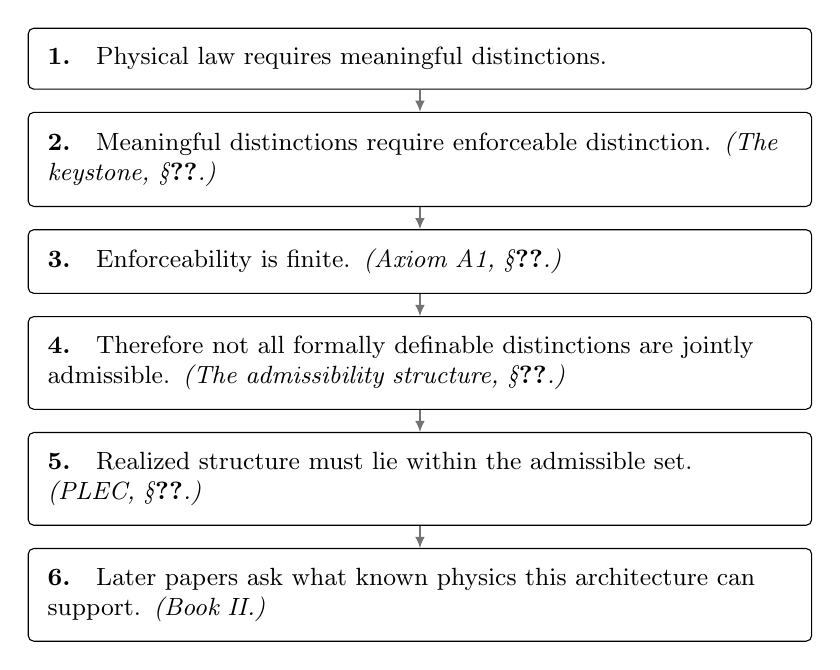
\begin{tikzpicture}[
    node distance=8pt,
    box/.style={
        rectangle,
        rounded corners=2pt,
        draw=black,
        line width=0.4pt,
        align=left,
        text width=0.78\linewidth,
        inner sep=7pt,
        font=\small
    },
    arrow/.style={-{Latex[length=4pt,width=3.5pt]}, line width=0.5pt, black!55}
]
\node[box] (n1) {\textbf{1.}\quad Physical law requires meaningful distinctions.};
\node[box, below=of n1] (n2) {\textbf{2.}\quad Meaningful distinctions require enforceable distinction. \emph{(The keystone, \S\ref{sec:keystone_claim}.)}};
\node[box, below=of n2] (n3) {\textbf{3.}\quad Enforceability is finite. \emph{(Axiom A1, \S\ref{sec:A1}.)}};
\node[box, below=of n3] (n4) {\textbf{4.}\quad Therefore not all formally definable distinctions are jointly admissible. \emph{(The admissibility structure, \S\ref{sec:admissibility_structure}.)}};
\node[box, below=of n4] (n5) {\textbf{5.}\quad Realized structure must lie within the admissible set. \emph{(PLEC, \S\ref{sec:PLEC}.)}};
\node[box, below=of n5] (n6) {\textbf{6.}\quad Later papers ask what known physics this architecture can support. \emph{(Book~II.)}};

\draw[arrow] (n1) -- (n2);
\draw[arrow] (n2) -- (n3);
\draw[arrow] (n3) -- (n4);
\draw[arrow] (n4) -- (n5);
\draw[arrow] (n5) -- (n6);
\end{tikzpicture}
\caption[The paper's logic chain]{\textbf{The paper's logic chain.} Each step is forced by the step above it under the reading that physical meaning requires enforceable distinction. The first five steps are the ontology this paper defends; step~6 marks the handoff to the downstream technical programme.}
\label{fig:logic_chain}
\end{figure}

\subsection{The keystone is not a theorem; and that is not a weakness}\label{sec:keystone_not_theorem}

The keystone is not derived within the framework. It is the commitment from which the framework's derivations begin. A reader accustomed to reductive programs may see this as a concession: the framework is not ``founded on pure logic'' or ``grounded in nothing.'' Two remarks.

First, every scientific framework rests on ontological commitments that are not internally derived. Classical mechanics rests on the commitment that positions exist. Quantum mechanics rests on the commitment that the probability amplitudes are physically interpretable. General relativity rests on the commitment that spacetime exists as a manifold. These commitments are not theorems \emph{of} their frameworks; they are the conditions under which those frameworks' theorems are meaningful. The keystone occupies the same structural slot.

Second, a virtue of stating the commitment clearly is that it can be argued about. Someone who rejects the keystone---who holds, for example, that physical distinctions can be meaningful without any cost of maintenance---rejects the framework, not a theorem inside it. That person has a clear attack surface: show an example of a physical distinction that persists with zero maintenance cost, or argue that the concept of maintenance cost is itself ill-posed. The framework's openness to that rejection is part of its strength: it locates its own foundations clearly enough to be attacked.

A third observation is more constructive. The keystone is not a dogmatic starting point; it is a structural one. It is the claim that resources limit physics before dynamics does, and that distinctions without resources are not physics. That claim is compatible with a wide range of more specific metaphysical positions. A reader with a different metaphysics of ``what exists'' can still accept the keystone's condition on \emph{when} a physical distinction is meaningful, and thereby engage with the framework's downstream results.

\clearpage

% ======================================================================
\section{The Finiteness of Enforcement (Axiom A1)}\label{sec:A1}
% ======================================================================

\subsection{From enforceable distinction to a capacity bound}\label{sec:A1_motivation}

The keystone commits the framework to the meaningfulness of distinctions that are actively enforced. The first structural consequence is that enforcement is not unlimited.

If enforcement cost were arbitrary---if any distinction could be maintained at any positive cost up to an unbounded budget---the keystone would deliver only a weak result: physical distinctions would exist, but the framework would have no way to predict which ones. Every admissible configuration would be equally admissible; the admissible set would be effectively the space of all finite-cost configurations.

The framework's predictive content comes from one further commitment: the total enforcement budget is finite. This is not derived from the keystone; it is added as a separate structural claim. The keystone says distinctions are meaningful only if maintained; \textbf{A1} says the total maintenance is bounded. Both are ontological commitments; they are independent.

\begin{tcolorbox}[apfbox, title={Axiom A1 --- Finite Enforcement Capacity}]
At any interface, the total enforcement cost committed across the maintained distinctions is bounded:
\[
\sum_{d \in G} \varepsilon(d) \leq C(\rho, \Gamma),
\]
where $G$ is the set of maintained distinctions, $\varepsilon(d)$ is the enforcement cost of distinction $d$, and $C(\rho, \Gamma)$ is the finite capacity of the interface defined by state $\rho$ and resource structure $\Gamma$.
\end{tcolorbox}

The formal statement encodes two claims: that enforcement cost is a real-valued function defined on distinctions (the cost exists and is finite), and that the total across all maintained distinctions at an interface is bounded (the capacity is finite). Together, these commit the framework to a bounded admissible set.

\Aone{} is not a theorem of anything more primitive. It is a structural claim about physics: the universe does not have unbounded resources for maintaining distinctions at any given interface. The claim is compatible with---indeed, supported by---a wide literature on finite information in physics: the Bekenstein--Hawking area bound~\cite{Bekenstein1981}, Landauer's principle~\cite{Landauer1961}, Ashby's Law of Requisite Variety~\cite{Ashby1956}. These results establish, in different settings, that finite physical systems support only finitely many distinctions. \Aone{} elevates the pattern to an ontological commitment.

Finiteness, in this setting, is not an auxiliary assumption layered atop the keystone. If enforceability were effectively unbounded, admissibility would become vacuous: any formally definable distinction could in principle be preserved jointly with arbitrarily many others, and the framework would lose the power to separate physically meaningful structure from unconstrained description. \Aone{} is what makes the keystone physically substantive. Removing finiteness does not leave a weaker version of the framework; it dissolves the framework altogether, because admissibility loses its bite.

\subsection{What A1 does}\label{sec:A1_does}

\Aone{} fixes the admissible set \emph{from above}. Without \Aone{}, the admissible set would be all configurations whose distinctions have positive finite cost; with \Aone{}, the admissible set is restricted to those whose total cost fits within the interface's capacity.

The restriction has downstream consequences that are easy to underestimate. It is \Aone{} that creates the competitive structure among distinctions: when the budget is finite, maintaining one distinction commits resources that cannot be committed elsewhere. That trade-off structure is what Papers~1 through~7 exploit. The superadditive cost surplus that Paper~1 derives---the cost of defending two overlapping distinctions exceeding the sum of the individual costs---is meaningful only under a finite budget. The non-closure of the admissibility algebra (Paper~2) is the algebraic consequence of competitive capacity use. The partition-function structure of APF (Paper~7) is a thermodynamic expression of the bounded capacity.

\Aone{}'s formal role, therefore, is to make admissibility a \emph{scarce} condition. Without it, any collection of finite-cost distinctions would be admissible; with it, admissibility becomes a non-trivial constraint, and the framework has content.

\subsection{What A1 does not do}\label{sec:A1_does_not}

\Aone{} is a precise claim, and its precision matters because the framework's downstream arguments depend on distinguishing what \Aone{} contributes from what other components contribute. Four clarifications.

First, \Aone{} does not rule out zero-cost distinctions. A distinction with $\varepsilon(d) = 0$ satisfies \Aone{} trivially (the cost adds nothing to the budget). The keystone excludes such distinctions on ontological grounds, and the companion axiom \textbf{MD} states the exclusion in the same form as \Aone{}---as a bound, now from below, rather than a hand-wave.

Second, \Aone{} does not select a realized configuration from the admissible set. The admissible set has, in general, many members; \Aone{} does not single one out. That role belongs to \textbf{A2}, the $\argmin$ component of the \emph{Principle of Least Enforcement Cost} (Ch.~4). A common failure mode in reading early drafts of the framework was to treat \Aone{} as if it did this work on its own---as if \Aone{}'s minimality were already the full variational principle. It is not; \Aone{} is a capacity bound, not a selection principle.

Third, \Aone{} does not impose variation in cost across distinctions. A world in which every distinction cost the same positive amount would satisfy \Aone{} (and \textbf{MD}), but the $\argmin$ would be uninformative: every admissible configuration with the same number of distinctions would tie. The framework therefore needs \textbf{BW}, the non-degeneracy condition, to ensure the cost spectrum is rich enough for the $\argmin$ to pick out a configuration.

Fourth, \Aone{} does not commit the framework to a specific value or scaling of capacity. The capacity $C(\rho, \Gamma)$ is interface-dependent; the framework's derivations use its existence and finiteness, not its specific value. The Bekenstein--Hawking area law is a physical instance of the capacity structure, but the keystone and \Aone{} do not \emph{presuppose} the area law; the area law is derived in Paper~3 from the admissibility structure.

Fifth, ``finite'' here does not mean negligible, perturbative, or uniformly small. It means only non-unbounded: distinctions must be sustained by physically commit-able structure, and therefore not every formally definable distinction can be jointly maintained without limit. A world with a very large but bounded capacity $C$ satisfies \Aone{} exactly as well as a world with a small capacity; what \Aone{} forbids is unbounded capacity, not large capacity. Readers who hear ``finite enforcement'' and infer ``small, local, perturbative'' should recalibrate: the framework does not assert that reality is weak, only that it is not unconstrained.

\subsection{The countermodel that separates A1 from MD}\label{sec:A1_countermodel}

The structural independence of \Aone{} from the positive-floor condition \textbf{MD} is important enough that Paper~1's Technical Supplement includes an explicit countermodel. We state it here because it is pivotal to the framework's ontological self-understanding.

Consider a one-dimensional interface with countably many distinctions $d_1, d_2, \dots$ with costs $\varepsilon(d_n) = 2^{-n}$. The total cost is $\sum_n 2^{-n} = 1$, which is finite. \Aone{} holds: the capacity bound $C = 1$ is satisfied by the full set of distinctions at arbitrarily high $n$. But \textbf{MD} fails: there is no positive lower bound on $\varepsilon(d_n)$, because $\inf_n \varepsilon(d_n) = 0$. The admissible set under \Aone{} alone admits the full sequence; the distinction at $d_n$ for large $n$ is arbitrarily close to a zero-cost distinction, which the keystone excludes.

The countermodel shows that \Aone{} does not imply \textbf{MD}: a world satisfying \Aone{} but violating \textbf{MD} is logically consistent and excluded only by the keystone acting through \textbf{MD}. The two components are therefore separate structural commitments; folding \textbf{MD} into \Aone{} is not an allowable shorthand.

The reverse direction is analogous: a world in which every distinction costs a positive minimum $\mu^* > 0$ but the total budget is unbounded would satisfy \textbf{MD} but violate \Aone{}, and the admissible set would be the full space of finite-distinction configurations---no scarcity, no predictive content. Each axiom excludes a different pathology; each is required.

The four-component independence picture (\Aone{}, \textbf{MD}, \textbf{A2}, \textbf{BW} all pairwise logically independent, each with its own countermodel) is developed in Paper~1 Supplement~\S1. Chapter~3 of this book returns to the picture with the companion components named.

\clearpage

% ======================================================================
\section{The Admissibility Structure}\label{sec:admissibility_structure}
% ======================================================================

\subsection{The admissible set as a structured object}\label{sec:admissible_set}

\Aone{} on its own produces a bounded set of configurations: those whose total cost fits within the interface's capacity. That set is not yet the admissibility structure of the framework. An admissibility structure is the bounded set \emph{together with} the conditions that make its geometry non-trivial: a lower bound on cost, a non-degeneracy condition on the cost spectrum, and the relational specification that ties costs at different distinctions together.

We name the structure as a whole first, then describe its components. At an interface specified by state $\rho$ and resource structure $\Gamma$, the \emph{admissibility structure} is the set
\[
\mathcal{A}(\rho, \Gamma) = \left\{\, G \;\Big|\; \varepsilon : G \to \mathbb{R}_{>0},\; \inf_{d \in G}\varepsilon(d) \geq \mu^*,\; \sum_{d \in G} \varepsilon(d) \leq C(\rho, \Gamma),\; \varepsilon \text{ non-degenerate} \,\right\}.
\]
The first condition (positivity of $\varepsilon$) is \textbf{MD}'s qualitative content; the second (positive infimum) is \textbf{MD} in its sharp form; the third is \Aone{}; the fourth is \textbf{BW}.

The admissibility structure is what the framework's downstream machinery operates on. When Paper~1 proves the superadditive cost surplus, it is proving a theorem about $\mathcal{A}$. When Paper~2 proves non-closure, it is proving that no single representation covers all of $\mathcal{A}$. When Paper~7 writes the APF partition function, the sum is over configurations in $\mathcal{A}$. The admissibility structure is the object of the framework, not \Aone{} in isolation.

\begin{figure}[h]
\centering
\includegraphics[width=0.78\textwidth]{Fig_Admissible_States_Diagram.pdf}
\caption{\textbf{The admissibility structure, visualized.} The
upper bulb is the admissible class
$\mathcal{A}(\rho, \Gamma)$ defined above: a bounded region in
correlation-capacity space, where ``everything is allowed'' inside the
boundary. The flanking shaded regions are not admissible: outside the
boundary, configurations either violate \Aone{} (the cost sum exceeds
$C(\rho, \Gamma)$) or violate \textbf{MD} (some distinction has zero or
sub-floor cost). The downward arrow labeled ``time'' is not yet present
in this paper --- it is the dynamical structure derived in
Paper~3. Time appears here as foreshadowing only: the picture this
paper makes static, Paper~3 makes dynamical. The narrowing near the
bottom (the ``locking interface'') is foreshadowing of Paper~5
measurement and Paper~6 regime exits; the three downstream tubes are
the $k!$ history sectors of Paper~5's $T9$. The bottom-right note
``capacity is a volume, entropy is an area'' anticipates Paper~3's
ledger result: entropy on a slice is the area-scaling of the
interface, not a literal two-dimensional surface. The diagram is
included here as the ontological frontispiece of the framework: every
later paper operates on some interpretation of this picture. Reading
the picture: the admissibility structure is what the rest of the
series studies; \Aone{}, \textbf{MD}, \textbf{BW}, and PLEC are the
four components by which the picture is given precise content.}
\label{fig:admissible-states}
\end{figure}

This figure will reappear, with paper-specific captions, in Papers~3,
6, and 7. Each paper interprets a different element of the picture:
Paper~3 derives the time arrow and the entropy slice; Paper~6
classifies the regime exits visible at the locking interface; Paper~7
turns the time-direction-through-the-volume into the action functional.

\subsection{MD --- the positive floor on distinction cost}\label{sec:MD}

\begin{tcolorbox}[apfbox, title={Axiom MD --- Minimum Distinction}]
Every physical distinction has strictly positive enforcement cost. There exists $\mu^* > 0$ such that, for every distinction $d$ in any admissible configuration,
\[
\varepsilon(d) \geq \mu^*.
\]
\end{tcolorbox}

\noindent \textbf{MD} is the keystone's exclusion of zero-cost distinctions, stated formally. It is a lower bound on the cost spectrum; \Aone{} is an upper bound on the cost sum. The two bounds together constrain the admissible set from both sides.

The logical independence of \textbf{MD} from \Aone{} is the countermodel of \S\ref{sec:A1_countermodel}: the sequence $\varepsilon(d_n) = 2^{-n}$ respects \Aone{} but violates \textbf{MD}, producing an admissible set contaminated by distinctions arbitrarily close to zero cost. The keystone excludes such distinctions on ontological grounds, and the exclusion has to be stated explicitly as an axiom because \Aone{} alone does not exclude them.

The value of $\mu^*$ is not specified. What matters is its strict positivity. In Paper~1, $\mu^*$ appears as the ``minimum cost floor'' of the theorem \textbf{L}$_{\varepsilon^*}$ (\emph{Minimum Cost Floor}, \coderef{check\_L\_epsilon\_star}{core.py}), whose value the downstream proofs do not exploit. The proofs exploit only that $\mu^* > 0$.

\textbf{MD}'s ontological role is to ensure the admissible set is populated by distinctions with real physical content. It is the condition under which the keystone's language of ``enforcement'' is not vacuous: distinctions have cost, and cost is bounded away from zero. Without \textbf{MD}, the admissible set would contain distinctions indistinguishable in the limit from their own absence; the keystone would then fail to deliver the content it promises.

\textbf{MD} is sometimes called the ``Stanford reviewer condition,'' because an early reviewer correctly noted that an earlier draft of the framework had been implicitly folding \textbf{MD} into \Aone{} and had to be repaired. The repair is preserved here: \textbf{MD} is named separately, its independence from \Aone{} is stated, and the countermodel is cited. Folding \textbf{MD} into \Aone{} is not an allowable shortcut.

\subsection{BW --- non-degeneracy of the cost spectrum}\label{sec:BW}

\begin{tcolorbox}[apfbox, title={Axiom BW --- Boundary Weight (Non-Degeneracy)}]
The enforcement cost $\varepsilon$ is non-degenerate on the admissible set: the cost spectrum is rich enough that, generically, configurations are separated by their total costs rather than identified.
\end{tcolorbox}

\noindent \textbf{BW} is the framework's structural condition on the \emph{variation} in cost across distinctions. Informally: in physics we should expect different distinctions to cost different amounts. Spin is not localization; charge is not mass; a nuclear binding energy is not an atomic ionization energy. The cost spectrum is rich.

\textbf{BW}'s role becomes clear in Chapter~4, when \textbf{A2} names the $\argmin$ as the realization locator. If the cost spectrum were degenerate---if, for some pair of configurations in $\mathcal{A}$, the total costs coincided---the $\argmin$ would not single out a configuration. The realized configuration would be ambiguous. \textbf{BW} is the commitment that this ambiguity does not occur generically; it commits the framework to a realized configuration that is, by the cost structure, uniquely selected.

The qualifier \emph{generically} matters. \textbf{BW} does not require that \emph{every} pair of configurations have distinct total cost; it requires that the cost spectrum be rich enough that the $\argmin$ is well-defined on the physically relevant admissible set. In finite regimes, the $\argmin$ can be verified directly; in continuous regimes, \textbf{BW} is the condition under which the $\argmin$ extends consistently. Paper~1's Supplement gives the precise statement; what matters for the ontology is the commitment that the cost spectrum is not degenerate by design.

\textbf{BW}'s independence from \Aone{} and \textbf{MD} is stated by a countermodel: a world in which every distinction costs exactly $\mu^*$, with total capacity $C$. Such a world satisfies \Aone{} and \textbf{MD} but has maximally degenerate cost spectrum; any two admissible configurations with the same number of distinctions tie in total cost. \textbf{BW} is the commitment that physics is not such a world.

\subsection{The four-layer hierarchy, stated}\label{sec:four_layer_hierarchy}

With the three structural components (\Aone{}, \textbf{MD}, \textbf{BW}) in hand, and \textbf{A2} still to be developed in Chapter~4, we can state the full ontological hierarchy of the framework. It has four layers, and they are ordered: each layer rests on the one below it.

\begin{tcolorbox}[apfbox, title={The Four-Layer Ontological Hierarchy}]
\begin{description}
    \item[Layer 1: The Keystone.] Meaning requires enforceable distinction.
    \item[Layer 2: Finiteness.] Enforcement is finite (\Aone{}).
    \item[Layer 3: Admissible Structure.] Admissible regimes are capacity-bounded and cost-structured (\Aone{}~$+$~\textbf{MD}~$+$~\textbf{BW}).
    \item[Layer 4: Realization.] The realized configuration is the $\argmin$ over the admissible set (\textbf{A2}; the \emph{Principle of Least Enforcement Cost} unifies all four components).
\end{description}
\end{tcolorbox}

\noindent The hierarchy is structural, not merely expositional. Each layer adds commitments that the previous layer does not deliver on its own. The keystone (layer 1) makes physical distinctions meaningful; it does not say how many can be enforced. \Aone{} (layer 2) makes the budget finite; it does not exclude zero-cost distinctions or distinguish the cost spectrum. \textbf{MD}~$+$~\textbf{BW} (layer 3) complete the structure of the admissible set; they do not single out a realized configuration. \textbf{A2} (layer 4) names the realization; it is the selection step the other three layers do not perform.

A common reading error is to collapse the four layers into a single ``foundational axiom.'' Earlier drafts of the framework sometimes did this, calling the whole structure ``finite enforceability of distinction'' and treating it as one principle. The reading is expositionally convenient and structurally wrong. Layer 1 is an ontological commitment (meaningfulness); layer 2 is a quantitative commitment (finiteness); layer 3 is a structural commitment (admissible-set geometry); layer 4 is a selection commitment (the $\argmin$). Each can be separately attacked. Each can be separately defended. Conflating them produces both strategic vulnerability (a reviewer attacking ``the axiom'' can hit any of four different things, each needing a different defense) and ontological vagueness (a reader cannot tell which layer is doing the work in a given derivation).

Papers~1 through~7 therefore do not speak of ``the axiom''; they speak of layers, components, or \PLEC{}'s four components. Paper~0 follows the same discipline.

\subsection{Structural independence of the four components}\label{sec:four_indep}

A final structural claim, important enough to state as a chapter-closer: the four components are pairwise logically independent.

Paper~1's Technical Supplement~\S1 proves this by exhibiting, for each component, a world that satisfies the other three and violates the one in question. The countermodels are concrete:

\begin{description}
    \item[\Aone{} alone violated:] $\varepsilon(d) = \mu^*$ for all $d$ (MD, BW, A2 satisfied), but $C = \infty$: no upper bound on the sum. The admissible set has unbounded cardinality; physics has no scarcity and no predictive content.
    \item[\textbf{MD} alone violated:] $\varepsilon(d_n) = 2^{-n}$. \Aone{} holds with $C = 1$; \textbf{BW} holds (the spectrum is rich, indeed too rich); \textbf{A2} is well-defined (the $\argmin$ exists). But \textbf{MD} fails: no positive infimum. The keystone is violated at the large-$n$ tail.
    \item[\textbf{BW} alone violated:] $\varepsilon(d) = \mu^*$ for all $d$ (\Aone{}, \textbf{MD}, \textbf{A2} satisfied in degenerate form). The cost spectrum is fully degenerate; the $\argmin$ is uninformative at the equal-count level.
    \item[\textbf{A2} alone violated:] \Aone{}, \textbf{MD}, \textbf{BW} all hold. The admissible set is well-specified. But realization does not sit at the $\argmin$: the framework selects from $\mathcal{A}$ by some other rule (uniform at random, maximal cost, some other functional). This is a coherent world; it is not \emph{this} framework.
\end{description}

\noindent Each countermodel shows that removing any single component collapses a different part of the framework. The four-component structure is not expositional redundancy; it is the minimal vocabulary in which the framework's commitments can be stated.

Chapter~4 now turns to \textbf{A2} itself and the \emph{Principle of Least Enforcement Cost} that unifies all four components.

\clearpage

% ======================================================================
\section{The Principle of Least Enforcement Cost}\label{sec:PLEC}
% ======================================================================

\subsection{From admissibility to realization}\label{sec:PLEC_from_admissibility}

Chapters~1 through~3 have established the admissibility structure: a keystone that makes distinctions meaningful, an \Aone{} that bounds the total cost from above, an \textbf{MD} that bounds individual costs from below, and a \textbf{BW} that keeps the cost spectrum non-degenerate. What we have so far is a characterization of the \emph{admissible set}---the set of configurations the framework takes to be physical candidates.

The admissible set is, in general, not a singleton. Many configurations share the same capacity, many respect the same cost floor, many are differentiated by the same non-degenerate spectrum. The framework's remaining ontological commitment is to say which of those configurations is \emph{realized}.

The commitment is that the realized configuration is the minimum-cost one.

\begin{tcolorbox}[apfbox, title={Axiom A2 --- Minimum-Cost Realization}]
At any interface $(\rho, \Gamma)$, the realized configuration is the $\argmin$ of total enforcement cost over the admissible set:
\[
G_{\mathrm{realized}}(\rho, \Gamma) = \argmin_{G \in \mathcal{A}(\rho, \Gamma)} \sum_{d \in G} \varepsilon(d).
\]
\end{tcolorbox}

\noindent The notation is standard: $\argmin$ names the element of $\mathcal{A}$ at which the cost sum attains its minimum. Under \textbf{BW}, the $\argmin$ is generically well-defined; ties are resolvable by the downstream uniqueness theorems of Papers~1 and~2 (tensor-product decomposition, anomaly cancellation, Witten parity), which the framework inherits from representation theory rather than adding as axioms.

\subsection{The canonical statement}\label{sec:PLEC_canonical}

\Aone{}, \textbf{MD}, \textbf{A2}, and \textbf{BW} are not four independent principles stated side-by-side. They are four components of a single variational principle---the condition on the admissible set (\Aone{}~$+$~\textbf{MD}~$+$~\textbf{BW}) combined with the selection operator on that set (\textbf{A2}). The framework names the unified principle the \emph{Principle of Least Enforcement Cost}.

\begin{tcolorbox}[apfbox, title={The Principle of Least Enforcement Cost (PLEC)}]
\textbf{Formal statement.} At every interface $(\rho, \Gamma)$, the realized configuration is
\[
G_{\mathrm{realized}}(\rho, \Gamma) = \argmin_{G \in \mathcal{A}(\rho, \Gamma)} \sum_{d \in G} \varepsilon(d),
\]
where the admissible set is
\[
\mathcal{A}(\rho, \Gamma) = \left\{\, G \;\Big|\; \inf_{d \in G} \varepsilon(d) \geq \mu^*,\; \sum_{d \in G} \varepsilon(d) \leq C(\rho, \Gamma),\; \varepsilon \text{ non-degenerate} \,\right\}.
\]
\textbf{Four structurally necessary components.}
\begin{description}
    \item[\Aone{}] (upper bound) --- the total cost is bounded by the interface capacity.
    \item[\textbf{MD}] (lower bound) --- each distinction costs at least $\mu^* > 0$.
    \item[\textbf{A2}] (argmin) --- realization is the minimum-cost admissible configuration.
    \item[\textbf{BW}] (non-degeneracy) --- the cost spectrum is rich enough for the argmin to be informative.
\end{description}
\textbf{Canonical lay statement.}
\begin{center}\itshape
Reality is the minimum-cost expression of distinction compatible with finite capacity.
\end{center}
\end{tcolorbox}

The lay statement is the frozen sentence the framework uses to name its content in one breath. It is placed verbatim on Paper~1 and Paper~13 as an epigraph; it is the opening of this paper and will be the closing of Ch.~16. It is not decoration; it is the single sentence from which the commitments of \PLEC{} are recoverable if all else is forgotten.

\subsection{The argmin is a locator, not a process}\label{sec:argmin_locator}

The single most common misreading of \PLEC{} is to treat the $\argmin$ as the output of an optimization \emph{process}. On this misreading, the framework describes a world in which something---nature, the universe, physical reality---is computing a minimum at each moment and delivering the result. That misreading imports an unstated dynamical and agential structure that the framework does not commit to. The term ``selection'' should not be read psychologically, computationally, or teleologically. It names a structural fact: among candidate continuations, only those compatible with finite enforceability belong to the physically realizable set. The extremal formulation is a compact representation of that admissible realized set, not a claim that nature executes an optimization routine.

The framework's ontological commitment is the opposite. The $\argmin$ is a \emph{locator}: it identifies where, inside the admissible set, the realized configuration sits. There is no optimizer, no search, no selection mechanism, no enforcer. The minimum is the referent of ``reality,'' not the output of a procedure that produces reality.

The analogy with classical mechanics is exact. In Hamilton's principle, the realized trajectory is the stationary point of the action functional over path space. Nothing in the principle commits to a process that finds the stationary point; the stationary point is what the realized trajectory \emph{is}, by definition. Cauchy problems deliver the trajectory as a dynamical evolution, but the variational characterization is independent of any such dynamics. \PLEC{} occupies the same structural slot at the admissibility level: the realized configuration is the $\argmin$, and that is what realization means.

This is why the descriptive-framing discipline of Chapter~5 is load-bearing. Language that narrates the $\argmin$ as an event---``reality selects the minimum,'' ``the system optimizes for X,'' ``the framework forces Y''---imports a process ontology the framework refuses. The framework's commitments are ontological and mathematical, not narrative.

\subsection{The scope of the argmin}\label{sec:argmin_scope}

\textbf{A2}'s $\argmin$ ranges over $\mathcal{A}(\rho, \Gamma)$: configurations \emph{already} admitted by the keystone, \Aone{}, \textbf{MD}, and \textbf{BW}. It does not reach outside the admissible set. Two implications follow.

First, configurations not in $\mathcal{A}$ do not compete with configurations in $\mathcal{A}$. A zero-cost configuration (excluded by \textbf{MD}) is not a ``cheaper'' option the $\argmin$ rejects; it is not an option at all. A configuration exceeding the capacity (excluded by \Aone{}) is not a ``more expensive'' option; it is outside the set on which the minimum is defined.

Second, the $\argmin$ is a local operator. At each interface $(\rho, \Gamma)$ the admissible set $\mathcal{A}(\rho, \Gamma)$ is specified; the $\argmin$ picks the minimum-cost member; the realized configuration at that interface is the result. The framework does not posit a global optimization across all interfaces; interface-locality is built into the structure. This is the content of the locality lemma \textbf{L}$_{\mathrm{loc}}$ (\coderef{check\_L\_loc}{core.py}) in Paper~1.

This scope-restriction forecloses a standing review challenge. A reviewer asking ``\PLEC{}'s minimum cost of what, relative to what admissible set?'' is asking a question the framework answers precisely: the minimum cost is of total enforcement across distinctions in $\mathcal{A}(\rho, \Gamma)$, and $\mathcal{A}(\rho, \Gamma)$ is specified by the keystone + \Aone{} + \textbf{MD} + \textbf{BW}. The admissible set is not a free parameter; it is fixed by the commitments of layers 1--3.

\subsection{PLEC in the variational tradition}\label{sec:PLEC_tradition}

\PLEC{} is a variational principle. The variational tradition in physics is long and well-understood: Fermat's principle of least time in optics (1662), Maupertuis's principle of least action in mechanics (1744), Hamilton's principle as the modern formulation (1834), Jaynes's maximum-entropy principle in statistical inference (1957), minimum free energy in thermodynamics. \PLEC{} belongs in this family. Its structural shape---a functional on a set of admissible configurations, with the realized configuration at the extremum---is recognizable to any physicist.

Where \PLEC{} differs is in what its admissible set is. The classical variational principles select among configurations \emph{already presumed populated}. Fermat's principle selects among paths through space; Hamilton's principle selects among trajectories in configuration space; Jaynes's principle selects among probability distributions over a pre-specified outcome space. None of these grounds the existence or structure of the configuration space they select over; each takes the space as given.

\PLEC{} does more. Its admissible set is defined by the framework's layers 1--3: configurations are admitted by the keystone, bounded in total cost by \Aone{}, bounded in individual cost by \textbf{MD}, and non-degenerate in spectrum by \textbf{BW}. \PLEC{} grounds both \emph{why} the space is populated (by the keystone and layers 2--3, which make physical distinctions meaningful and admissibility a non-trivial condition) and \emph{what within it is realized} (by layer~4, the $\argmin$). This is the sense in which \PLEC{} ``does more'' than the classical variational principles: it operates on an admissible set that the principle itself---through its four components---specifies.

\subsection{Non-merge discipline}\label{sec:non_merge}

A virtue of the four-component decomposition is that it allows \PLEC{} to be unified at the level of presentation while keeping the components structurally separate. \Aone{}, \textbf{MD}, \textbf{A2}, \textbf{BW} are four features of one principle; they are not four independent axioms stated side-by-side.

This unification, however, must not collapse into a merger. Each component is logically independent of the other three (\S\ref{sec:four_indep}); each is defended by its own countermodel; each ontological attack on the framework targets one or more of the four, not an amorphous ``axiom.'' The non-merge discipline is therefore:

\begin{itemize}
    \item The framework presents \PLEC{} as a single variational principle, for pedagogical clarity and for positioning in the variational tradition.
    \item The framework names and defends \Aone{}, \textbf{MD}, \textbf{A2}, \textbf{BW} as separate components, for logical rigor and reviewer-facing transparency.
    \item The framework does not collapse \textbf{MD} into \Aone{}, or \textbf{A2} into \Aone{} (both collapses were made in earlier drafts and have been explicitly repaired), or \textbf{BW} into a regularity condition on some other component.
\end{itemize}

\noindent The practical consequence: any attribution of a downstream result to ``the axiom'' is imprecise. Downstream results are attributable to specific components. When Paper~2 derives $N_c = 3$, the derivation uses \Aone{} (capacity bound), \textbf{MD} (positive floor), and \textbf{A2} ($\argmin$); it does not use \textbf{BW} essentially, and it does not depend on any specific value of $\mu^*$. The four-component vocabulary makes such attributions possible. The unified-axiom vocabulary does not.

\clearpage

% ======================================================================
\section{Descriptive Reading}\label{sec:descriptive_reading}
% ======================================================================

\subsection{The convention, stated}\label{sec:descriptive_convention}

\PLEC{} is a statement about where the realized configuration sits inside the admissible set. It is not a statement about a process that \emph{puts} the realized configuration there. The admissibility conditions (\Aone{}, \textbf{MD}, \textbf{BW}) are conditions on a set; the $\argmin$ (\textbf{A2}) is an operator on that set. Nothing in the four components commits the framework to an optimizer, a selector, an enforcer, or an agent.

This descriptive reading is not a nicety. It is the difference between a framework that commits to what it commits to, and a framework that imports unstated commitments through its narrative. The history of variational physics is instructive: Hamilton's principle has repeatedly been misread as ``nature chooses the path of least action,'' despite every formal treatment of the principle insisting that the ``choice'' is a locator, not a process. The misreading is usually harmless in classical mechanics, because the reader can inspect the differential equations that the variational principle is equivalent to and see that no process is being described. In an ontology paper, the misreading would be structural: it would grant the framework a selection mechanism the framework refuses.

The convention this paper follows, and that the companion technical papers follow in their framing boxes (Paper~1~\S2.0, Paper~2~\S2.0, Paper~13~\S2.3), is:

\begin{tcolorbox}[apfbox, title={Descriptive Reading Convention}]
Throughout the framework, statements of the form
\begin{itemize}
    \item ``X is uniquely admissible,''
    \item ``The admissibility conditions admit only X,''
    \item ``X is the $\argmin$ over the admissible set,''
    \item ``Y is excluded by the admissibility conditions,''
\end{itemize}
are \emph{locator statements}: they identify where realized configurations sit inside the admissibility structure. They do not describe a process, a mechanism, a choice, or an agent. No enforcer is being posited; no dynamics is being evoked. The admissible set is what it is; the $\argmin$ is what it is; realization is the logical consequence of those two structural facts.
\end{tcolorbox}

\subsection{Why this convention matters}\label{sec:descriptive_why}

A framework that commits to an enforcer or an optimizer has additional ontological load: it has to explain what the enforcer is, where it comes from, how it operates, and why it selects the minimum rather than any other functional. A framework that commits to \PLEC{} as a locator has no such load: the admissible set's structure and the $\argmin$ are the framework's content, and nothing more is being claimed.

This is a strict minimalism. The framework does not claim that reality ``computes'' the minimum, or that some physical substrate is implementing the optimization, or that a meta-dynamics is searching for the $\argmin$. These would be additional commitments on top of \PLEC{}'s four components; the framework refuses them.

There is a second, equally important reason for the discipline. The downstream uniqueness theorems of Papers~1 and~2 are consumed incorrectly if they are read as selection processes. When Paper~2 proves ``the gauge template $SU(3)\times SU(2)\times U(1)$ is uniquely admissible,'' the claim is that this template is the single member of the admissible set under the framework's structural conditions; no other template is admitted. It is \emph{not} the claim that the framework ``chose'' the Standard Model's gauge group out of some pool of alternatives. The latter reading invites ``why this and not that?''-type objections that apply to selection processes; the former reading invites the different (and framework-friendly) question ``is the admissible set correctly specified?''

The descriptive reading therefore is not stylistic. It is substantive: it determines what the framework commits to and what attacks it is vulnerable to. A reader trained in the descriptive reading can engage with the framework on its actual content. A reader who narrates the framework's results as a selection process will critique a framework the framework does not claim to be.

A related misreading, worth naming explicitly, is to treat the framework as a dressed-up operationalism in the narrow epistemic sense. The present view is not reducible to that. It does not define reality by what an observer happens to measure. It defines physical meaning by what the world can sustain as a distinction, whether or not any particular observer is present. Observation is one mode of realized enforcement, not the definition of meaning. The emphasis is ontological before it is epistemic: the framework commits to what the world supports, and only secondarily to how that support is detected.

\subsection{How this paper uses language}\label{sec:descriptive_language}

The discipline is applied sentence-by-sentence through the rest of this volume, not as a global flag. Four specific rewrites recur:

\begin{description}
    \item[``X forces Y''] becomes ``Y is uniquely admissible under X'' or ``the conditions induced by X admit only Y'' or ``Y is the $\argmin$ over the set $\mathcal{A}$ specified by X.'' The translation is not cosmetic: it names the admissible set whose uniqueness or minimum is being asserted.
    \item[``The system selects X''] becomes ``X is the realized configuration at this interface'' or ``X is the $\argmin$ over the admissible set at this interface.'' Where the selection-language is an established idiom in the underlying mathematics (as in ``gauge selection''), the idiom is preserved but flagged at its first use.
    \item[``Reality chooses X''] becomes ``X is realized''---full stop, no choice-language. If a reader wants to know \emph{why} X is realized, the answer is: X is the $\argmin$ over the admissible set, and realization is defined as occupying the $\argmin$.
    \item[``Nature optimizes for X''] becomes ``X is the $\argmin$ of the relevant cost functional over the admissible set'' or, more often, is struck: the optimization-language is a leftover from selection-process narration and usually contributes nothing the locator-language does not deliver more precisely.
\end{description}

\noindent A small residual category of selective language is retained for readability and is flagged inline. ``Forces,'' ``selects,'' and ``admits'' all appear in the framework's technical papers and in some sections of Book~II of this volume; where they appear, they are locator-shorthand, not process-claims. The reader is asked to read them that way throughout.

\subsection{An applied glossary}\label{sec:glossary}

A short translation table for the most common admissibility-phrasings. The right column is always a statement about a structured set and a locator; the left column is narrative shorthand.

\begin{center}
\begin{tabular}{p{0.45\linewidth}p{0.45\linewidth}}
\toprule
\textbf{Narrative phrasing} & \textbf{Descriptive translation}\\
\midrule
``The framework forces $SU(3) \times SU(2) \times U(1)$.'' & ``$SU(3) \times SU(2) \times U(1)$ is the unique gauge template in the admissible set under the framework's structural conditions.''\\
\addlinespace
``Finite capacity forces noncommutativity.'' & ``The admissible enforcement algebra admits no faithful commutative representation under \Aone{}~$+$~\textbf{MD}~$+$~\textbf{BW}.''\\
\addlinespace
``Measurement collapses the superposition.'' & ``At measurement, the admissibility conditions narrow the admissible set until only one outcome remains; the superposed configuration leaves the admissible set.''\\
\addlinespace
``The system chooses $N_c = 3$.'' & ``$N_c = 3$ is the unique color-group rank in the admissible set under cost-minimization.''\\
\addlinespace
``Nature forbids composite fermions at zero cost.'' & ``Composite fermions at zero cost are excluded from the admissible set by \textbf{MD}.''\\
\addlinespace
``Reality selects the minimum-cost configuration.'' & ``Reality is the minimum-cost configuration; no selection is performed, and none is required.''\\
\bottomrule
\end{tabular}
\end{center}

\noindent The translations are not style changes. Each right-column entry names \emph{what} is admissible, \emph{what} conditions specify the admissible set, and \emph{where} the realized configuration sits. Each left-column entry leaves those questions implicit or wrong.

\subsection{The descriptive reading and the Book II chapters}\label{sec:descriptive_bookII}

Book~II of this volume has one chapter per technical paper, and each chapter includes a sub-section (``Where `forces' is a descriptor'') that applies the discipline of Chapter~5 to that paper's specific selective-language. This is where the conventions of this chapter earn their keep: every place a technical paper uses ``forces,'' ``selects,'' or ``admits,'' the Book~II chapter translates the phrasing into the admissibility-language above.

The reader should not take the translations as corrections to the technical papers. The papers use selective-language where it is clearer than locator-language, and each paper has its own framing box stating the descriptive reading. Book~II's translations make the two readings explicit: a reader can see the paper's chosen phrasing and its locator-equivalent side by side, and confirm that the paper is committing to the locator-interpretation.

With the conventions in place, we now turn to the papers themselves.

\clearpage

% ======================================================================
\part{Derivational Commitments}
% ======================================================================

\noindent Book~II states, for each technical paper, what the paper derives and what ontological commitments the derivation draws on. Each chapter follows a fixed six-section template:

\begin{quote}
\S X.1 Scope. \hspace{2em} \S X.2 Ontological commitments drawn on. \hspace{2em} \S X.3 Structural results, stated not proved. \hspace{2em} \S X.4 Where ``forces'' is a descriptor. \hspace{2em} \S X.5 What the paper does not claim. \hspace{2em} \S X.6 Status at current codebase version.
\end{quote}

\noindent Chapters~6--8 and~12 cover papers that are mature (Papers 1, 2, 3, 7) and are written in full. Chapters~9--11 and~13 cover papers that are mature in codebase content but await a .tex rewrite (Papers 4, 5, 6) or are reserved (Paper 8); they are placeholder chapters whose structure will be preserved as content fills in. Each placeholder states what the codebase currently establishes, citing the relevant check functions, so the chapter is usable by a current reader.

% ======================================================================
\section{Paper 1: The Enforceability of Distinction}\label{sec:P1}
% ======================================================================

\subsection{Scope}\label{sec:P1_scope}

\paperref{1}{The Enforceability of Distinction} is the formal spine of the framework. It states the four-component structure of \PLEC{} formally, proves pairwise logical independence of the components, develops the cost-based foundations (enforcement cost $\varepsilon$, locality \textbf{L}$_{\mathrm{loc}}$, minimum cost floor \textbf{L}$_{\varepsilon^*}$), establishes the superadditive cost surplus from which noncommutativity of the enforcement algebra follows, and delivers the quantum reconstruction: a finite-dimensional complex Hilbert space, the Born rule (via Gleason), and the Tsirelson bound $2\sqrt{2}$.

The paper is, at v4.0-PLEC, approximately 40~pages with an 81-page Technical Supplement. Its scope includes both the ontological commitments (which this book's Chapter~1--5 transliterates at the ontology-paper level) and the downstream mathematics that converts those commitments into quantum structure.

\subsection{Ontological commitments drawn on}\label{sec:P1_commitments}

Paper~1 draws on all four layers of the ontological hierarchy. Specifically:

\begin{itemize}
    \item \textbf{Layer 1 (keystone).} Paper~1's title names this layer; its abstract and~\S1 state it as the ontological foundation of the framework.
    \item \textbf{Layer 2 (\Aone{}).} Paper~1~\S2.0--\S2.1 presents \Aone{} as the finiteness axiom; \S2.2--\S2.3 develops the formal structure of enforcement cost and the capacity bound.
    \item \textbf{Layer 3 (\textbf{MD}, \textbf{BW}).} Paper~1~\S2.3 states \textbf{MD} as the minimum-cost floor; the Supplement~\S1 develops \textbf{BW} as the non-degeneracy of the cost spectrum and provides the independence countermodel.
    \item \textbf{Layer 4 (\textbf{A2}).} Paper~1~\S2.4 states \textbf{A2} as the $\argmin$ operator; the Supplement~\S1 proves that \textbf{A2} is not derivable from \Aone{} + \textbf{MD} alone (the explicit countermodel is the world where realization is uniform-at-random over $\mathcal{A}$).
\end{itemize}

\noindent Paper~1 also makes use of FD1--FD6, the \emph{Finite Distinction} set of constitutive principles, which are derived rather than axiomatized: they specify how enforcement cost interacts with distinction composition, additivity, and locality. These are not additional ontological commitments; they are consequences of the layers above, established as propositions within the paper.

\subsection{Structural results}\label{sec:P1_results}

Paper~1's main results, stated without proof:

\begin{description}
    \item[Locality of capacity ($\mathbf{L}_{\mathrm{loc}}$).] Enforcement capacity is interface-local: $C(\rho, \Gamma)$ is specified at each interface, independent of the configuration at spacelike-separated interfaces. \coderef{check\_L\_loc}{core.py}
    \item[Minimum cost floor ($\mathbf{L}_{\varepsilon^*}$).] Every admissible distinction has $\varepsilon(d) \geq \mu^* > 0$. This is \textbf{MD} in theorem form within the local-interface setting. \coderef{check\_L\_epsilon\_star}{core.py}
    \item[Superadditive cost surplus ($\mathbf{L}_\Delta$).] The cost of defending two overlapping distinctions exceeds the sum of their individual costs. This is the load-bearing superadditivity from which noncommutativity follows. \coderef{check\_L\_nc}{core.py}
    \item[Order-dependence theorem ($\mathbf{T}_1$).] The residual budget after enforcing distinction~$A$ before~$B$ differs from the residual after enforcing~$B$ before~$A$, under the superadditive surplus. Order-dependence is therefore observable.
    \item[Noncommutative algebra theorem ($\mathbf{T}_{\mathrm{alg}}$).] The enforcement algebra admits no faithful commutative representation. \coderef{check\_L\_nc}{core.py}
    \item[Wedderburn--Artin structure ($\mathbf{T}_{2a}$).] The enforcement algebra decomposes into a direct sum of matrix algebras over division rings. \coderef{check\_T\_canonical}{core.py}
    \item[Complex field selection ($\mathbf{T}_{2c}$).] The division ring of the enforcement algebra is $\mathbb{C}$ (not $\mathbb{R}$, not $\mathbb{H}$), by two proved exclusions $P_{\mathrm{tom}}$ (tomographic) and $P_{\mathrm{cls}}$ (closure). \coderef{check\_T\_canonical}{core.py}
    \item[GNS representation ($\mathbf{T}_{\mathrm{GNS}}$).] The algebra admits a faithful representation on a Hilbert space. \coderef{check\_T\_alg}{core.py}
    \item[Born rule ($\mathbf{T}_{\mathrm{Born}}$).] Probabilities of measurement outcomes are squared amplitudes, by Gleason applied to the cost-derived measure on projections. \coderef{check\_T\_Born}{core.py}
    \item[Tsirelson bound ($\mathbf{T}_{\mathrm{Tsirelson}}$).] CHSH correlations are bounded by $2\sqrt{2}$, from the tensor structure of independent interfaces. \coderef{check\_T\_Tsirelson}{core.py}
\end{description}

\noindent The Technical Supplement extends this list with proofs and additional results including interface monogamy, no-broadcasting, and the Bloch--Redfield-style decoherence threshold.

\subsection{Where ``forces'' is a descriptor}\label{sec:P1_forces}

Paper~1 uses selective-language in four load-bearing contexts, and each is translatable into locator-language. The translations are not corrections to the paper; they confirm that the paper's selective-phrasings are consumed descriptively.

\begin{itemize}
    \item ``\Aone{} \emph{forces} noncommutativity'' (Paper~1 abstract, \S1) $\longmapsto$ ``the admissible enforcement algebra, under \Aone{} + \textbf{MD} + \textbf{BW}, admits no faithful commutative representation; noncommutativity is the unique admissible algebra structure.''
    \item ``Superadditivity \emph{forces} order-dependence'' (Paper~1 \S4) $\longmapsto$ ``the admissible cost functional under superadditive surplus does not commute across distinct enforcement orderings; the residual budgets after $(A, B)$ and $(B, A)$ differ as a theorem, not as a contingency.''
    \item ``The complex field is \emph{selected} by proved theorems'' (Paper~1 abstract) $\longmapsto$ ``under the admissibility structure of \Aone{} + \textbf{MD} + \textbf{BW}, the only division ring compatible with $P_{\mathrm{tom}}$ and $P_{\mathrm{cls}}$ is $\mathbb{C}$; $\mathbb{R}$ and $\mathbb{H}$ are excluded.''
    \item ``Cost minimization \emph{selects} the quantum skeleton'' (Paper~1 \S5) $\longmapsto$ ``the quantum skeleton is the $\argmin$ over the admissible set under \PLEC{}; no other admissible configuration has lower total cost.''
\end{itemize}

\noindent In each case the locator-language names the admissible set whose uniqueness or minimum is being asserted, and commits the paper to no selection process.

\subsection{What Paper 1 does not claim}\label{sec:P1_does_not_claim}

Paper~1's scope is bounded. It does not claim, and should not be read as claiming:

\begin{itemize}
    \item \emph{Specific particle content.} Fermion generations, gauge group, field content are Paper~2's and Paper~4's scope. Paper~1 establishes the quantum reconstruction; it does not specify what particles populate the Hilbert space.
    \item \emph{Absolute scale of capacity.} The capacity $C(\rho, \Gamma)$ is interface-local and finite; its specific value is not fixed by Paper~1. (It is fixed, where it is fixed, by downstream papers' counting arguments, notably Paper~2's $C_{\mathrm{total}} = 61$.)
    \item \emph{Value of $\hbar$.} The minimum quantum of action is developed in Paper~7; Paper~1 establishes the structural existence of noncommutative structure without committing to its numerical scale.
    \item \emph{Interpretation of measurement as a dynamical event.} Paper~1's measurement theory is structural: it derives the probability law (Born) and the algebraic framework, not a process-level account of collapse. Collapse as dynamics is not a claim Paper~1 defends.
    \item \emph{Independence from the four-component structure.} Paper~1 does not claim \Aone{} alone suffices for its results. The Supplement's countermodels explicitly show that removing any of \Aone{}, \textbf{MD}, \textbf{A2}, \textbf{BW} collapses a different part of the derivation.
\end{itemize}

\subsection{Status at current codebase version}\label{sec:P1_status}

Paper~1 is at v4.0-PLEC (April 2026). The version fully adopts \PLEC{} as the canonical variational formulation, names all four components, and has the Supplement essentiality proofs anchored. The paper is 40~pages of main body and 81~pages of Supplement. It has been reviewed twice internally; it is targeted for submission to \emph{Foundations of Physics}. Its downstream consumption by Papers~2--7 is live: all subsequent papers draw on Paper~1's definitions and theorems rather than re-deriving them.

\clearpage

% ======================================================================
\section{Paper 2: The Structure of Admissible Physics}\label{sec:P2}
% ======================================================================

\subsection{Scope}\label{sec:P2_scope}

\paperref{2}{The Structure of Admissible Physics} (folder name: ``Structure and Gauge Uniqueness'') takes Paper~1's quantum reconstruction and determines the structural content of the admissibility algebra at global scale. It proves the \emph{non-closure theorem}: no single representation of the admissibility algebra covers all admissibility regimes. It then identifies the gauge-template structure that is uniquely admissible: $SU(3) \times SU(2) \times U(1)$, with $N_c = 3$ and the 45-fermion spectrum that Paper~4 enumerates in detail. Three structural predictions follow: $\theta_{\mathrm{QCD}} = 0$, vacuum stability, proton stability. Two cosmological fractions: $\Omega_\Lambda = 42/61$, $\Omega_m = 19/61$. One precision prediction: $\sin^2\theta_W = 3/13$.

The paper is, at v5.3-PLEC, approximately 47~pages with a 96-page Technical Supplement.

\subsection{Ontological commitments drawn on}\label{sec:P2_commitments}

Paper~2 draws on layers 1--4 as transmitted through Paper~1. It imports:

\begin{itemize}
    \item The keystone (layer 1) and \Aone{} (layer 2), from Paper~1~\S2.
    \item The admissibility structure \Aone{} + \textbf{MD} + \textbf{BW} (layer 3), from Paper~1~\S2.
    \item \PLEC{}'s argmin (\textbf{A2}, layer 4), from Paper~1~\S2.4.
    \item Paper~1's quantum reconstruction: the noncommutative algebra, the Hilbert-space representation, the complex field.
\end{itemize}

\noindent Paper~2 additionally commits to two hypotheses the framework names but does not derive:

\begin{description}
    \item[Sharing-admissibility (S).] The admissibility structure allows configurations in which distinct subsystems share resource commitments. This is the condition under which tensor products exist; without it, the framework collapses to independent interfaces with no composite structure.
    \item[Generation-channel hypothesis (GCH).] The framework admits a generation-channel bridge connecting distinct ``copies'' of a representational structure to yield observed generational multiplicity. This underwrites the argument that $N_{\mathrm{gen}} = 3$ is structurally forced rather than contingent.
\end{description}

\noindent Both hypotheses are flagged at point of use in Paper~2 and its Supplement. Paper~0's commitment is to the framework's layers 1--4; Paper~2's hypotheses S and GCH are downstream ontological choices that the framework could in principle repair if either were challenged, and Paper~0 does not absorb them into its layer structure.

\subsection{Structural results}\label{sec:P2_results}

Paper~2's main results, stated without proof:

\begin{description}
    \item[Non-closure theorem.] The admissibility algebra does not close on any single representation: for every representation compatible with admissibility at a given interface, there exist admissibility regimes at which that representation fails. No global representation covers all of admissibility. \coderef{check\_T\_Tsirelson}{core.py}
    \item[Gauge template uniqueness ($\mathbf{L}_{\mathrm{gauge\_template}}$).] $SU(3) \times SU(2) \times U(1)$ is the unique gauge template in the admissible set under the non-closure constraints, with $N_c \geq 3$ forced by the colored-structure argument. \coderef{check\_L\_gauge\_template\_uniqueness}{gauge.py}
    \item[Color-group rank ($\mathbf{T}_{\mathrm{gauge}}$).] $N_c = 3$ is the unique argmin of total cost over admissible color-group ranks; $N_c = 2$ fails non-closure, $N_c \geq 4$ exceeds capacity at fixed cost per generator. \coderef{check\_T\_gauge}{gauge.py}
    \item[Field content ($\mathbf{T}_{\mathrm{field}}$).] Of 4,680 potential fermion templates compatible with the gauge structure, exactly one survives the admissibility constraints (anomaly cancellation, Witten parity, capacity-budget). The surviving template is the 45-fermion Standard Model content. \coderef{check\_T\_field}{gauge.py}
    \item[Capacity count ($\mathbf{L}_{\mathrm{count}}$).] The total capacity count is $C_{\mathrm{total}} = 45 + 4 + 12 = 61$: 45 fermions, 4 electroweak, 12 strong-force channels.
    \item[Three structural predictions.] $\theta_{\mathrm{QCD}} = 0$ (strong CP admits only the zero value at zero cost), vacuum stability (the admissible vacuum is stable under perturbations), proton stability (the admissible proton is the lowest-cost baryon in its sector).
    \item[Cosmological fractions ($\mathbf{L}_{\mathrm{equip}}$).] Horizon equipartition yields $\Omega_\Lambda = 42/61$ and $\Omega_m = 19/61$. Observational values: $\Omega_\Lambda = 0.6847 \pm 0.0073$, $\Omega_m = 0.3153 \pm 0.0073$ (Planck+BAO). Framework prediction matches within $0.05\%$ and $1.2\%$ respectively.
    \item[Weak mixing angle ($\mathbf{L}_{\mathrm{Cauchy}}$, $\mathbf{T}_{\gamma}$).] $\sin^2\theta_W = 3/13 \approx 0.2308$, from the Cauchy-uniqueness chain $F(d) = d \to \gamma = 17/4 \to \sin^2\theta_W = 3/13$. Observed value: $0.2312 \pm 0.0002$. Agreement within $0.2\%$.
    \item[Cabibbo angle.] $\sin\theta_C = e^{-3/2} \approx 0.2231$. Observed: $0.2245 \pm 0.0008$. Agreement within $0.6\%$. \coderef{check\_L\_Gram\_generation}{generations.py}
\end{description}

\subsection{Where ``forces'' is a descriptor}\label{sec:P2_forces}

Paper~2 uses selective-language in six recurring contexts.

\begin{itemize}
    \item ``The admissibility algebra \emph{does not close}'' $\longmapsto$ ``no single representation is admissible across all admissibility regimes; the admissible set of global representations is empty.''
    \item ``The gauge template is \emph{forced}'' $\longmapsto$ ``$SU(3) \times SU(2) \times U(1)$ is the unique gauge template in the admissible set under the non-closure conditions.''
    \item ``$N_c = 3$ is \emph{selected}'' $\longmapsto$ ``$N_c = 3$ is the $\argmin$ over admissible color-group ranks; ranks $\neq 3$ are either excluded by non-closure or exceed capacity.''
    \item ``The framework \emph{rules out} additional generations'' $\longmapsto$ ``four or more generations exceed $C_{\mathrm{total}}$; such configurations are outside the admissible set.''
    \item ``$\theta_{\mathrm{QCD}} = 0$ is \emph{required}'' $\longmapsto$ ``$\theta_{\mathrm{QCD}} = 0$ is the admissible value at zero enforcement cost; $\theta \neq 0$ is admissible only at positive cost $\varepsilon^* > 0$, which \textbf{A2} declines.''
    \item ``Anomaly cancellation \emph{selects} the surviving template'' $\longmapsto$ ``of 4,680 gauge-compatible templates, exactly one is in the admissible set after anomaly, parity, and capacity-budget constraints; this is the Standard Model template.''
\end{itemize}

\subsection{What Paper 2 does not claim}\label{sec:P2_does_not_claim}

Paper~2's scope is bounded in several ways.

\begin{itemize}
    \item \emph{Absolute mass scale.} Paper~2 derives mass \emph{ratios} and structural predictions, not absolute masses. The mass scales $m_t$, $m_b$ in particular are Type-B anchors whose absolute value requires a derivation of the cost-scale $\sigma$; this is an open problem.
    \item \emph{Dark matter identity.} Paper~2 establishes that $C_{\mathrm{total}} = 61$ and the admissible cosmological fractions, but does not identify a specific particle for dark matter. Paper~3 and Paper~6 develop dark-matter structure; neither commits to a particle ID.
    \item \emph{Generation mass ordering beyond structural ratios.} Paper~2 derives the structural form of the generation mass spectrum; specific mass values for $m_c$ (known to be at $2.6\%$ from observation, at the Schur structural limit) are open.
    \item \emph{BSM mechanisms.} Paper~2 catalogs the admissible template; it does not extend to BSM physics. BSM mechanisms are named conservatively in Paper~7 (seesaw, etc.) without quantitative claims.
\end{itemize}

\subsection{Status at current codebase version}\label{sec:P2_status}

Paper~2 is at v5.3-PLEC (April 2026). The version adopts \PLEC{} as the canonical formulation, propagates the four-component vocabulary from Paper~1, and carries all structural results at current codebase v6.8. Paper~2 has been through two audit passes (the descriptive-framing pass and the eight-finding Non-Closure and Gauge audit) with all findings A--H applied. It is 47~pages of main body and 96~pages of Supplement. It is ready for submission alongside Paper~1.

\clearpage

% ======================================================================
\section{Paper 3: Entropy, Time, and Accumulated Cost}\label{sec:P3}
% ======================================================================

\subsection{Scope}\label{sec:P3_scope}

\paperref{3}{Entropy, Time, and Accumulated Cost} develops entropy in the framework without a probability primitive. Entropy is the count of admissible configurations consistent with the macroscopic state; the arrow of time is the irreversibility of admissible-configuration transitions; records are accumulated enforcement cost. Paper~3 v3.0 (April 2026) extends the scope with \emph{admissibility carrying capacity} (ACC) as the general-capacity concept of which enforcement cost is the quantum-interface specialization; derives horizon entropy $S = A/4$ from a $1/2 \times 1/2$ bookkeeping argument (relational double-counting plus Hamiltonian-constraint gauge redundancy); introduces the \emph{ledger-accounting principle} (entropy as a count robust under cost-landscape corrections); and develops staged cosmogenesis (constraint functional $\Phi_c = \ln(d_{\mathrm{field}}/d_{\mathrm{admissible}})$, overconstrained initial regime, staged relaxation).

At v3.0 the paper is 23~pages.

\subsection{Ontological commitments drawn on}\label{sec:P3_commitments}

Paper~3 draws on all four ontological layers as transmitted through Paper~1, and additionally commits to:

\begin{description}
    \item[The ledger-accounting principle.] Entropy is a count of admissible configurations. It is robust under interaction corrections and thermal $\beta$-shifts because multiplicity is insensitive to cost-landscape details. This is a commitment about \emph{what entropy is}, not a theorem: it declines the Shannon-entropy framing and declines the statistical-mechanical derivation from a probability primitive. Papers~1 and~2 do not use this commitment; Paper~3 is where it enters.
    \item[Staged relaxation.] The admissible set does not populate all at once. The constraint functional $\Phi_c$ is monotone along admissible trajectories; the early universe sits in an overconstrained regime with $\Phi_c$ large, and the admissible set grows through a sequence of stage-transitions. This commitment underwrites the framework's cosmogenesis picture.
\end{description}

\noindent Both commitments are flagged at point of use in Paper~3 as framework-level rather than derivation-local.

\subsection{Structural results}\label{sec:P3_results}

\begin{description}
    \item[Entropy as admissible count.] Entropy $S$ is $\ln$ of the number of admissible microconfigurations consistent with the macrostate; no probability primitive is needed.
    \item[Ledger-accounting principle.] Entropy is robust under cost-landscape corrections: interaction terms and thermal $\beta$-shifts do not change the count of admissible configurations.
    \item[Arrow of time.] Macroscopic irreversibility is the loss of global admissible coordination, not a contingent low-entropy initial condition. \coderef{check\_T\_second\_law}{supplements.py}
    \item[Low-entropy initial state.] The early universe's low entropy is structural (restricted admissible phase space), not improbable. The typicality argument is rebutted structurally rather than statistically.
    \item[Admissibility carrying capacity (ACC).] Horizon capacity is an instance of admissibility capacity at the geometric level; enforcement cost is the quantum-interface specialization.
    \item[Horizon entropy ($\mathbf{T}_{\mathrm{deSitter\_entropy}}$).] $S = A/4$, derived from $1/2 \times 1/2$ bookkeeping: half for relational double-counting, half for Hamiltonian-constraint gauge redundancy. \coderef{check\_T\_horizon\_reciprocity}{gravity.py}
    \item[Constraint functional ($\Phi_c$).] $\Phi_c = \ln(d_{\mathrm{field}}/d_{\mathrm{admissible}})$ is monotone along admissible trajectories; provides the entropy bound and staged-relaxation structure.
    \item[Staged cosmogenesis.] The early universe's admissible set is overconstrained; staged relaxation produces scale-dependent imprints and the inflation-era admissibility structure.
    \item[Trapped-surface threshold.] Horizon enforceability admits a trapped-surface criterion; below threshold, geometry holds; above threshold, admissibility fails geometry-first.
\end{description}

\subsection{Where ``forces'' is a descriptor}\label{sec:P3_forces}

\begin{itemize}
    \item ``Saturation \emph{forces} the horizon'' $\longmapsto$ ``at saturation the admissible set is restricted to configurations with horizon-boundary topology; non-horizon configurations are outside the admissible set.''
    \item ``The arrow of time is \emph{forced} by irreversibility'' $\longmapsto$ ``the admissible set of forward transitions is strictly larger than the admissible set of reverse transitions; reverse transitions are generically outside the admissible set, not selected against by a process.''
    \item ``Cosmogenesis \emph{drives} the admissible set to grow'' $\longmapsto$ ``along admissible trajectories, $\Phi_c$ decreases monotonically; the admissible set expands through stage-transitions as the constraint functional relaxes.''
\end{itemize}

\subsection{What Paper 3 does not claim}\label{sec:P3_does_not_claim}

\begin{itemize}
    \item \emph{Quantitative pre-big-bang cosmology.} Paper~3 develops the structural cosmogenesis picture; quantitative pre-inflation cosmology is deferred to Paper~6.
    \item \emph{Horizon corrections beyond $1/2 \times 1/2$.} The paper commits to the first-order bookkeeping; higher-order corrections are deferred to Paper~6 and Paper~7.
    \item \emph{Dark matter identity.} Paper~3 develops the framework-level dark-matter commitments (existence, properties from $T_{12}$) but does not identify a particle.
    \item \emph{Specific inflation model.} Paper~3 commits to staged relaxation and constraint-functional monotonicity; specific inflation-era observables are deferred to Paper~6.
\end{itemize}

\subsection{Status at current codebase version}\label{sec:P3_status}

Paper~3 is at v3.0 (April 2026). The version incorporates the scope expansion for Geometric Carrying Capacity, Cosmogenesis and Staged Relaxation, and the ledger-accounting principle, plus two additional falsifiers (F4 ringdown memory / horizon enforceability; F5 structured pre-saturation imprints). The partition-function cross-reference to Paper~7 is live: Paper~3~\S5 now forward-references Paper~7's thermodynamic formalism. The paper is 23~pages and compiles cleanly at codebase v6.8.

\clearpage

% ======================================================================
\section{Paper 4: Admissibility Constraints and Field Content}\label{sec:P4}
% ======================================================================

\begin{tcolorbox}[pendingbox, title={Status: placeholder chapter}]
This chapter is a placeholder at Paper~0 v3.0. Paper~4's technical rewrite (from PDF to .tex) is pending; when the rewrite lands, this chapter will fill out the six-section template in full. Until then, the chapter states scope and the commitments Paper~4 currently carries at codebase v6.8.
\end{tcolorbox}

\subsection{Scope}\label{sec:P4_scope}

\paperref{4}{Admissibility Constraints and Field Content} (folder name: ``Constraints - Field Content and Fermion Spectrum'') enumerates the fermion spectrum of the Standard Model from the admissibility structure: the 45 fermions in three generations, their quantum numbers, and the admissibility-level constraints (anomaly cancellation, Witten parity, generation-channel bridge, sector decomposition) that select the surviving template. Paper~4 also derives $N_{\mathrm{gen}} = 3$ and the associated generation-mixing structure, and develops mass structure through the Schur-limit argument.

\subsection{Ontological commitments drawn on}\label{sec:P4_commitments}

Paper~4 draws on all four ontological layers, as transmitted through Papers~1 and~2, and additionally commits to:

\begin{itemize}
    \item The generation-channel hypothesis (GCH) from Paper~2, used here for $N_{\mathrm{gen}} = 3$.
    \item The sharing-admissibility hypothesis (S) from Paper~2, used here for composite structure.
\end{itemize}

\noindent No new framework-level commitments are introduced.

\subsection{Structural results (codebase v6.8; full statements pending .tex rewrite)}\label{sec:P4_results}

\begin{description}
    \item[Fermion count.] 45 fermions total (15 per generation $\times$ 3 generations). \coderef{check\_T\_field}{gauge.py}
    \item[Generation count.] $N_{\mathrm{gen}} = 3$, from the capacity-ladder argument under \Aone{} + \textbf{MD} + \textbf{A2}. \coderef{check\_T7}{gauge.py}
    \item[1-of-4,680.] The Standard Model template is the unique admissible survivor of 4,680 gauge-compatible candidate templates under anomaly, parity, and capacity constraints.
    \item[Mass-ratio structure.] Generation mass ratios follow a Schur-structural chain; $m_c$ at 2.6\% from observation is the framework's structural limit and an open problem.
    \item[Cabibbo angle.] $\sin\theta_C = e^{-3/2}$, in agreement with PDG.
    \item[CKM matrix structure.] The CKM matrix structure is constrained by the generation-channel bridge; full element-by-element derivation is the \coderef{check\_T\_CKM}{generations.py} scope.
\end{description}

\subsection{Where ``forces'' is a descriptor (pending .tex)}\label{sec:P4_forces}

Translation table to be filled in when Paper~4 .tex is produced. The current codebase uses selective-language primarily in two contexts: ``the admissibility structure \emph{forces} $N_{\mathrm{gen}} = 3$'' (locator-equivalent: ``$N_{\mathrm{gen}} = 3$ is the $\argmin$ of total cost over admissible generation counts'') and ``anomaly cancellation \emph{selects} the surviving template'' (locator-equivalent: handled in Paper~2~\S\ref{sec:P2_forces}).

\subsection{What Paper 4 does not claim}\label{sec:P4_does_not_claim}

\begin{itemize}
    \item \emph{Absolute mass scales.} $m_t$ and $m_b$ are Type-B anchors; absolute scale requires a $\sigma$ derivation that remains open.
    \item \emph{Neutrino mass hierarchy.} Paper~4 commits to the Type-I seesaw mechanism (developed in Paper~7); specific hierarchy predictions are open.
    \item \emph{Extra generations.} Paper~4 excludes $N_{\mathrm{gen}} \geq 4$ structurally; no hidden-generation speculation is entertained.
\end{itemize}

\subsection{Status at current codebase version}\label{sec:P4_status}

Paper~4 is currently PDF-only; no editable .tex source exists. The codebase at v6.8 carries all structural results above. When a .tex rewrite is produced, this chapter will extend the four-sub-sections above into full form, the descriptive-framing translation table will be completed, and the chapter's placeholder status will be lifted.

\clearpage

% ======================================================================
\section{Paper 5: Quantum Structure from Finite Enforceability}\label{sec:P5}
% ======================================================================

\begin{tcolorbox}[pendingbox, title={Status: placeholder chapter}]
This chapter is a placeholder at Paper~0 v3.0. Paper~5's role in the series is currently under review: much of its original scope has been absorbed by Paper~1 v4.0-PLEC. This chapter states the scope that remains, for reference.
\end{tcolorbox}

\subsection{Scope}\label{sec:P5_scope}

\paperref{5}{Quantum Structure from Finite Enforceability} historically developed Hilbert space, the Born rule, tensor products, and measurement structure from admissibility. Paper~1's v4.0 rewrite absorbed the quantum reconstruction (Hilbert space, complex field, Born rule, Tsirelson bound), leaving Paper~5 with a narrower remaining scope: CPTP formalism, specific decoherence results, tensor-product measurement structure for composite systems, and the interaction of measurement with the admissibility breakdown at measurement interfaces.

\subsection{Ontological commitments drawn on}\label{sec:P5_commitments}

Paper~5 draws on layers 1--4 as transmitted through Paper~1. It additionally commits to the Sharing-admissibility hypothesis (S) of Paper~2 for tensor-product structure on composites.

\subsection{Structural results (codebase v6.8; .tex rewrite pending)}\label{sec:P5_results}

\begin{description}
    \item[CPTP formalism.] Completely positive trace-preserving maps arise as the admissible evolution class on composite systems. \coderef{check\_T\_CPTP}{core.py}
    \item[Tensor-product structure.] Composite admissibility yields tensor-product Hilbert spaces under S.
    \item[Measurement-interface breakdown.] At measurement, the admissibility conditions narrow the admissible set; Paper~5 develops the structure of this narrowing as a conditional on the macroscopic interface.
\end{description}

\subsection{Where ``forces'' is a descriptor (pending .tex)}\label{sec:P5_forces}

To be filled in when Paper~5's remaining scope is finalized and the .tex is written.

\subsection{What Paper 5 does not claim}\label{sec:P5_does_not_claim}

Paper~5 does not re-derive Paper~1's quantum reconstruction; it extends it to composite and measurement-interface contexts.

\subsection{Status at current codebase version}\label{sec:P5_status}

Paper~5 is currently PDF-only; scope is under review in light of Paper~1 v4.0's absorption of quantum reconstruction. When Paper~5's remaining scope is finalized, this chapter will be rewritten accordingly.

\clearpage

% ======================================================================
\section{Paper 6: Dynamics and Geometry}\label{sec:P6}
% ======================================================================

\begin{tcolorbox}[pendingbox, title={Status: placeholder chapter}]
This chapter is a placeholder at Paper~0 v3.0. Paper~6's technical rewrite is pending; the codebase carries the structural results.
\end{tcolorbox}

\subsection{Scope}\label{sec:P6_scope}

\paperref{6}{Dynamics and Geometry as Optimal Admissible Reallocation} (folder name: ``Dynamics and Geometry - Spacetime and Gravity'') derives the Einstein equations from admissibility under Lovelock uniqueness in $d=4$, the geodesic structure from cost-minimizing paths, the cosmological-constant structure from horizon equipartition, and the DESI-era dynamical dark-energy commitments. Paper~6 also covers the Coleman--Mandula theorem, HKM causal-order structure, and Malament full-metric recovery.

\subsection{Ontological commitments drawn on}\label{sec:P6_commitments}

Paper~6 draws on layers 1--4 via Paper~1. It additionally commits to:

\begin{itemize}
    \item The chartability condition (geometric interfaces admit local coordinatization).
    \item The causal-order commitment (admissible transitions respect a partial order).
    \item The Lovelock uniqueness condition (admissible curvature tensors are linear in $R_{\mu\nu}$ in $d=4$).
\end{itemize}

\noindent These are downstream structural commitments, not framework-level axioms.

\subsection{Structural results (codebase v6.8; .tex rewrite pending)}\label{sec:P6_results}

\begin{description}
    \item[Einstein equations uniqueness.] In $d=4$, Lovelock admits only the Einstein tensor; the admissible curvature structure is $R_{\mu\nu} - (1/2) R g_{\mu\nu} + \Lambda g_{\mu\nu} = \kappa T_{\mu\nu}$. \coderef{check\_A9\_closure}{gravity.py}
    \item[Geodesic motion.] Admissible paths in a capacity gradient are geodesics of the induced metric.
    \item[Cosmological structure.] $\Omega_\Lambda = 42/61$ and $\Omega_m = 19/61$ from horizon equipartition (derived in Paper~2, used in Paper~6's cosmological-scale context).
    \item[DESI tension.] The framework's $w = -1$ commitment is in 2.8--4.2$\sigma$ tension with DESI DR1 dynamical dark-energy signals; Paper~6 develops the framework's position on the tension.
    \item[Coleman--Mandula.] The admissible spacetime symmetries decompose into the direct product of the Lorentz group and internal symmetry, by admissibility-level argument independent of the S-matrix construction.
\end{description}

\subsection{Where ``forces'' is a descriptor (pending .tex)}\label{sec:P6_forces}

To be completed when .tex rewrite is produced.

\subsection{What Paper 6 does not claim}\label{sec:P6_does_not_claim}

\begin{itemize}
    \item \emph{Quantum gravity interior.} Paper~6 develops the framework's classical-geometry commitments; admissibility breakdown at the Planck scale is Paper~7 territory.
    \item \emph{Dark matter identity.} Cosmological fractions come out; particle ID is open.
    \item \emph{DESI resolution.} The DESI tension is acknowledged; a resolution is not yet committed.
\end{itemize}

\subsection{Status at current codebase version}\label{sec:P6_status}

Paper~6 is currently PDF-only. Structural results are carried by the codebase; .tex rewrite pending. DESI DR2/DR3 developments are being watched.

\clearpage

% ======================================================================
\section{Paper 7: Action, Internalization, and the Lagrangian}\label{sec:P7}
% ======================================================================

\subsection{Scope}\label{sec:P7_scope}

\paperref{7}{Action, Internalization, and the Lagrangian} is the framework's bridge between the ontological layers developed in Papers~1--3 and the Standard Model Lagrangian. It has five parts. Part~I (\emph{Quantum of Action}) establishes a minimum action floor $\varepsilon^*$ below which no admissible record can be formed, and the \emph{Isolation of Zero} theorem separating the zero-action configuration from all non-zero admissible ones. Part~II (\emph{Partition Function}) writes the APF partition function $Z_0(\beta) = (1 + d_{\mathrm{eff}} e^{-\beta \varepsilon^*})^{C_{\mathrm{total}}}$, identifies the gapped-ground-state regime $kT \ll \varepsilon^*$ with a 10$^{32}$~margin below the Planck scale, and states the saturation factorisation $Z_{\mathrm{sat}} = N_{\mathrm{micro}} \cdot \exp(-\beta E_{\mathrm{sat}}(\eta))$. Part~III (\emph{Spectral Action = APF Partition Function}) proves the four-step identity between the Connes spectral action $\mathrm{Tr}[f(D/\Lambda)]$ and the APF partition function at a Boltzmann cutoff; the Seeley--DeWitt expansion with $a_0 = 61$, $a_2 \approx 21.985$, $a_4 \approx 87.201$ produces the cosmological constant, Einstein--Hilbert gravity, Yang--Mills, and Higgs-potential terms of the Standard Model Lagrangian. Part~IV (\emph{Geometric Internalization}) develops the Kolmogorov continuum, chartability, Lovelock-uniqueness, Coleman--Mandula, HKM causal-order uniqueness, and Malament full-metric recovery as stand-alone arguments within the framework. Part~V (\emph{SM Lagrangian Extensions}) derives the one-loop $\beta$-coefficients $b_1 = 41/10$, $b_2 = -19/6$, $b_3 = -7$ from APF field content, the Type-I seesaw, Pauli--Jordan spin-statistics, the McKean--Singer index theorem, and the Tannaka--Krein reconstruction of $SU(3) \times SU(2) \times U(1)$.

Paper~7 v2.0 is 21~pages of main paper with a 17-page Technical Supplement.

\subsection{Ontological commitments drawn on}\label{sec:P7_commitments}

Paper~7 draws on all four ontological layers and additionally commits to three hypotheses flagged at point of use:

\begin{description}
    \item[H1 (spectral-triple ansatz).] The admissibility structure at a Lorentzian interface admits a spectral-triple representation $(A, H, D)$ with a finite-dimensional algebra $A$, a Hilbert space $H$, and a Dirac operator $D$ whose spectrum encodes the admissible cost functional. This is not derived from layers 1--4; it is a compatibility commitment between admissibility and Connes' noncommutative-geometry machinery.
    \item[H2 (Lipschitz cost regularity).] The cost functional $\varepsilon$ is Lipschitz on the admissible set, uniformly in the capacity parameter. This is the regularity condition under which the argmin operator commutes with the Seeley--DeWitt expansion.
    \item[H3 (HKM future-distinguishing).] The admissible causal structure is future-distinguishing: distinct events have distinct admissible futures. This is the condition under which the HKM theorem applies to admissibility-induced causal-order.
\end{description}

\noindent Each hypothesis is flagged in the paper at its point of use; Paper~0's commitment is to the framework's layers 1--4, and Paper~7's three additional hypotheses are downstream ontological choices that could in principle be repaired or replaced.

\subsection{Structural results}\label{sec:P7_results}

\begin{description}
    \item[MD-floor / $\varepsilon^*$-floor (\textbf{Lemma 1.1}, \textbf{Theorem 1.2}).] Every admissible record commits at least $\varepsilon^*$ of enforcement cost. Below $\varepsilon^*$ no admissible record forms.
    \item[Isolation of Zero (\textbf{Theorem 1.3}).] The zero-cost configuration is isolated from the admissible set: there is no continuous deformation of an admissible record into the zero-record; the transition is structural.
    \item[$k!$ multi-record (\textbf{Theorem 1.4}).] Multi-record configurations carry a $k!$ combinatorial factor from admissibility-consistent orderings.
    \item[Closed-form partition function (\textbf{Theorem 2.1}).] $Z_0(\beta) = (1 + d_{\mathrm{eff}} e^{-\beta \varepsilon^*})^{C_{\mathrm{total}}}$, with $d_{\mathrm{eff}} = 102$ the effective self-exclusion dimension and $C_{\mathrm{total}} = 61$ the capacity count. \coderef{check\_L\_spectral\_action\_internal}{internalization.py}
    \item[Gapped-ground-state regime (\textbf{Theorem 2.3}).] For $kT \ll \varepsilon^*$, the partition function is dominated by the ground-state contribution; with $\varepsilon^* \sim E_P$, this regime covers the full observable universe with margin $\sim 10^{32}$.
    \item[Saturation factorisation (\textbf{Theorem 3.2}).] $Z_{\mathrm{sat}}(\beta, \eta) = N_{\mathrm{micro}} \cdot \exp(-\beta E_{\mathrm{sat}}(\eta))$, where $N_{\mathrm{micro}} = d_{\mathrm{eff}}^{C_{\mathrm{total}}}$ is a count and $E_{\mathrm{sat}}(\eta)$ is a configuration-dependent energy. Directly satisfies Paper~3~\S5's forward-reference for thermodynamic formalism.
    \item[Spectral action = APF partition function (\textbf{Theorem 4.2}).] Under H1, the Connes spectral action $\mathrm{Tr}[f(D/\Lambda)]$ equals the APF partition function at a Boltzmann cutoff. This is the structural pivot of the paper.
    \item[Seeley--DeWitt expansion (\textbf{Theorem 4.3}).] The spectral-action expansion in $\Lambda^{-1}$ has coefficients $a_0 = 61$, $a_2 \approx 21.985$, $a_4 \approx 87.201$. These produce the cosmological constant, Einstein--Hilbert term, Yang--Mills term, and Higgs potential of the Standard Model Lagrangian.
    \item[Uniqueness of the spectral action (\textbf{Theorem 4.4}).] The spectral action is the unique admissible action satisfying (U1) spectral invariance, (U2) gauge invariance, (U3) positivity, (U4) cutoff regularisation, and \textbf{A2} argmin.
    \item[One-loop $\beta$-coefficients.] $b_1 = 41/10$, $b_2 = -19/6$, $b_3 = -7$ from APF field content at the electroweak scale. \coderef{check\_T6B\_beta\_one\_loop}{extensions.py}
    \item[Type-I seesaw.] The neutrino mass mechanism is admissible under the framework's field-content structure; see \coderef{check\_L\_seesaw\_type\_I}{extensions.py}.
    \item[Pauli--Jordan spin-statistics.] The admissible spin-statistics connection is derived from admissibility, not imposed.
    \item[McKean--Singer index theorem.] The chiral anomaly structure follows from admissibility at the spectral level.
    \item[Tannaka--Krein $\to SU(3) \times SU(2) \times U(1)$.] The gauge group is reconstructed from the admissibility-induced tensor category, independently of Paper~2's argument.
\end{description}

\subsection{Where ``forces'' is a descriptor}\label{sec:P7_forces}

\begin{itemize}
    \item ``The spectral action \emph{is} the APF partition function'' $\longmapsto$ ``under H1, the two functionals agree on the admissible set; no distinct action is admissible.''
    \item ``Seeley--DeWitt \emph{produces} the SM Lagrangian'' $\longmapsto$ ``the first four Seeley--DeWitt coefficients reconstruct the admissible Lagrangian structure uniquely: the cosmological constant, Einstein--Hilbert, Yang--Mills, and Higgs terms are the admissible Lagrangian content at this order.''
    \item ``The framework \emph{forces} $b_1 = 41/10$'' $\longmapsto$ ``$b_1 = 41/10$ is the unique admissible one-loop coefficient under the APF field content; other values are excluded by admissibility.''
    \item ``Tannaka--Krein \emph{selects} $SU(3) \times SU(2) \times U(1)$'' $\longmapsto$ ``the admissible tensor category's Tannaka--Krein reconstruction is $SU(3) \times SU(2) \times U(1)$; this is the unique admissible gauge structure at the tensor-category level.''
\end{itemize}

\subsection{What Paper 7 does not claim}\label{sec:P7_does_not_claim}

\begin{itemize}
    \item \emph{Numerical value of $\hbar$.} Paper~7 establishes the minimum quantum of action structurally; its numerical value depends on the universe's specific capacity budget, which is not fixed within Paper~7.
    \item \emph{Quantitative BSM predictions.} BSM mechanisms (seesaw structure, beyond-SM sector content) are named conservatively without quantitative claims. Paper~7 is explicit that Part~V names mechanisms, not numerics.
    \item \emph{Saturation exactness as a substantive claim.} The saturation factorisation is a factorisation, not an ``exactness theorem.'' Paper~7's Supplement~\S7 flags this: $N_{\mathrm{micro}}$ is a count, and counts do not depend on cost-landscape details, but this is tautological rather than substantive. The substantive content is the factorisation itself; the framework does not use ``exact'' as a marketing claim for the framework's cosmological-constant prediction.
    \item \emph{$\Lambda \cdot G$ is exact.} The correct statement is ``$\Lambda \cdot G$ is forced by counting, not tuned''; the counting ingredients themselves ($C_{\mathrm{total}} = 61$, $d_{\mathrm{eff}} = 102$) are structurally forced by upstream arguments, not by Paper~7.
\end{itemize}

\subsection{Status at current codebase version}\label{sec:P7_status}

Paper~7 is at v2.0 (April 2026). The version replaces the February~2026 PDF-only v1.0 (6~pages on minimum action) with a full-scope rewrite absorbing PLEC framing, partition function, saturation factorisation, spectral-action internalization, geometric internalization, and SM Lagrangian extensions. The v2.0 main paper is 21~pages; the Technical Supplement is 17~pages. Both compile cleanly. Paper~3 v3.0's forward-reference to Paper~7 for thermodynamic formalism is now live and satisfied.

\clearpage

% ======================================================================
\section{Paper 8: Correlation Space (reserved)}\label{sec:P8}
% ======================================================================

\begin{tcolorbox}[pendingbox, title={Status: reserved slot}]
This chapter is a placeholder for Paper~8, which is reserved in the series but has no substantive content committed at Paper~0 v3.0. When Paper~8's scope and results are developed, this chapter will fill out the six-section template. Until then, this chapter exists to preserve the series structure.
\end{tcolorbox}

\subsection{Scope (reserved)}\label{sec:P8_scope}

Paper~8 is reserved for content on correlation space: the structural space of admissible correlations between interfaces, and its relation to the framework's information-geometric structure. Specific scope is yet to be committed.

\subsection{Ontological commitments (reserved)}\label{sec:P8_commitments}

To be determined by Paper~8's eventual scope. Any framework-level commitments beyond layers 1--4 will be flagged here when the paper is written.

\subsection{Structural results (reserved)}\label{sec:P8_results}

Pending Paper~8.

\subsection{Where ``forces'' is a descriptor (reserved)}\label{sec:P8_forces}

Pending Paper~8.

\subsection{What Paper 8 does not claim (reserved)}\label{sec:P8_does_not_claim}

Pending Paper~8.

\subsection{Status}\label{sec:P8_status}

Reserved slot. No current .tex, no current PDF; codebase does not yet carry Paper~8-specific content.

\clearpage

% ======================================================================
\part{The Framework in the World}
% ======================================================================

% ======================================================================
\section{Where Standard Physics Lives}\label{sec:regimes}
% ======================================================================

\subsection{Regime scoping, not replacement}\label{sec:regime_scoping}

The framework does not claim to replace classical mechanics, quantum mechanics, general relativity, thermodynamics, or quantum field theory. The framework is the containing structure within which each of these is regime-valid. The relationship is compositional: the framework specifies admissibility; the standard theories operate within admissible regimes.

This is not a hedge. It is a structural claim. Each standard theory is associated with an admissibility regime in which its representation is faithful---the admissibility conditions supporting the theory's equations hold in that regime, and the theory's predictions match the framework's admissibility-level predictions. Outside the regime, the representation fails. The framework predicts \emph{where} each standard theory is valid, and \emph{where} it breaks down.

Six standard regimes are examined in the sections that follow. Each is characterized by the admissibility conditions that support it, the specific representational structure that holds in the regime, and the conditions under which the regime breaks.

\subsection{Where quantum mechanics lives}\label{sec:where_QM}

Quantum mechanics is the representation of admissibility in regimes where:

\begin{itemize}
    \item bilinearity of the correlation structure holds (independent-interface tensor products exist);
    \item saturation is sparse (most interfaces operate below capacity; capacity gradients are gentle);
    \item records have not locked (the admissible set has not narrowed to a single outcome at the macroscopic scale).
\end{itemize}

\noindent In such regimes, the framework's noncommutative algebra (\textbf{T}$_{\mathrm{alg}}$, Paper~1) admits a faithful Hilbert-space representation; amplitudes obey the Born rule (\textbf{T}$_{\mathrm{Born}}$, Paper~1); and interferences between admissible configurations are observable. The representation fails at measurement interfaces (where the admissible set narrows to one outcome) and at the high-capacity / saturated regime (where the algebra's closure fails non-trivially, per Paper~2).

The measurement problem, in this reading, is not a problem. It is a regime-transition: an interface at which the admissibility conditions supporting the unitary representation cease to hold, and the representation exits its domain of validity. No ``collapse'' as a dynamical event is posited; no ``observer'' is posited. Measurement is where the admissibility conditions narrow $\mathcal{A}$ until only one configuration remains.

\subsection{Where spacetime geometry lives}\label{sec:where_GR}

Classical Lorentzian geometry is the representation of admissibility in regimes where:

\begin{itemize}
    \item capacity redistributes smoothly across the interface (no sharp capacity gradients);
    \item saturation is sparse (most regions operate below capacity);
    \item integrability holds locally (paths admit a length functional whose extremization is well-defined).
\end{itemize}

\noindent In such regimes, the admissibility structure supports a metric representation: capacity gradients are encoded as curvature; cost-minimizing paths are geodesics; Einstein's equations follow from the Lovelock-uniqueness argument in $d=4$ (Paper~6). The representation fails at horizons (where the admissibility conditions supporting integrability break, per Paper~3's horizon enforceability) and at singularities (where admissibility fails geometry-first).

Black holes, in this reading, are not exotic objects. They are regions where admissibility saturates locally: the geometric representation exits its domain of validity. The information paradox, as classically posed, assumes the geometric representation extends across the horizon. The framework's answer is that the representation does not extend; what happens ``inside'' the horizon is not a geometric fact but an admissibility-level fact that must be treated in its own terms.

\subsection{Where thermodynamics lives}\label{sec:where_thermo}

Thermodynamics is the representation of admissibility in regimes where:

\begin{itemize}
    \item many distinctions interact (the admissible set is combinatorially rich);
    \item records have formed (the admissible set at the macroscale has narrowed);
    \item reversal is inadmissible (the admissible set of reverse transitions is strictly smaller than forward transitions).
\end{itemize}

\noindent In such regimes, entropy is the logarithm of the admissible-microconfiguration count consistent with the macroscopic state (Paper~3); the second law is the structural statement that the admissible set of forward transitions exceeds the admissible set of reverse transitions; the arrow of time is the resulting asymmetry. Temperature, free energy, chemical potential emerge as descriptors of the admissibility structure's shape, not as substantive quantities beyond it.

The ledger-accounting principle (Paper~3~\S5) makes this scoping precise: the entropy count is robust under cost-landscape corrections. Small changes in enforcement-cost details do not shift the entropy, because the count is not sensitive to them. Thermodynamics is therefore stable in its regime: its predictions are insulated from the framework's microstructural details.

\subsection{Where action principles live}\label{sec:where_action}

Action-principle formulations (Hamilton, Lagrangian, path-integral) are the representation of admissibility in regimes where:

\begin{itemize}
    \item admissible neighborhoods exist (small variations around each configuration are in $\mathcal{A}$);
    \item cost is locally additive along paths (the path-integrated cost functional exists);
    \item extrema are unique (the $\argmin$ over path space is well-defined).
\end{itemize}

\noindent In such regimes, the Euler--Lagrange equations are the local form of \textbf{A2}; the action functional is the local representation of the enforcement-cost sum; the path-integral is the partition function at zero temperature. The representation fails where admissibility is not locally smooth (at topology-change, at measurement, at singularities) and where cost ceases to be locally additive (at saturated regimes).

Paper~7's spectral-action = APF partition function identity makes the representation explicit at the field-theoretic level: the Standard Model Lagrangian, from which Hamilton's principle delivers the equations of motion, is the Seeley--DeWitt expansion of the admissibility partition function. The action principle is therefore not primitive; it is the representation of admissibility at regimes where the Seeley--DeWitt expansion converges.

\subsection{Where the classical limit lives}\label{sec:where_classical}

Classical mechanics is the representation of admissibility in regimes where:

\begin{itemize}
    \item records have locked at the macroscopic scale (the admissible set at the macroscale is effectively a single configuration);
    \item the Born-rule weighting concentrates on a single outcome (amplitudes for alternative outcomes are negligible);
    \item the geometric representation holds smoothly.
\end{itemize}

\noindent In such regimes, classical trajectories are the unique admissible paths; quantum alternatives are suppressed; the representation reduces to Newton or Hamilton as appropriate. The classical limit is a regime within the quantum regime; it is not a pre-quantum theory the framework subordinates.

\subsection{What the framework does not change}\label{sec:framework_no_change}

The regime-scoping picture has negative content that deserves stating.

\begin{itemize}
    \item \emph{Within each regime, the standard theory is correct.} The framework does not revise Maxwell's equations within the classical-electrodynamics regime, or the Schr\"odinger equation within the unitary-evolution regime, or the Einstein equations within the smooth-geometry regime. These are regime-correct; the framework inherits their content.
    \item \emph{No hidden variables.} The framework does not introduce local hidden variables underneath quantum mechanics. Bell's theorem is respected: the framework's admissibility structure is non-local in the sense required.
    \item \emph{No new forces within-regime.} Within each regime, the framework does not predict new in-regime phenomena beyond what the standard theory covers. New predictions are regime-boundary phenomena: where one representation breaks down and another takes over.
    \item \emph{No overthrow of observational physics.} The framework is compatible with, and reproduces, all confirmed observational physics. Where it makes novel predictions, the predictions are specific and falsifiable (see Chapter~15); where it overlaps with known physics, it reproduces the known results.
\end{itemize}

\noindent This scoping is, in one sense, conservative. The framework does not undo physics; it organizes it. But the organization itself has content: where standard theories break down (measurement, horizons, singularities, cosmogenesis, high-capacity regimes), the framework provides admissibility-level answers that the standard theories do not.

\clearpage

% ======================================================================
\section{Status, Predictions, Falsifiers}\label{sec:status}
% ======================================================================

\subsection{The codebase as authoritative specification}\label{sec:codebase}

The framework's authoritative specification is not this paper, nor any of the technical papers individually. It is the APF codebase, currently at \textbf{v6.8 (frozen 2026-04-18, Phase 2.9 canonicalization pass)}. The codebase carries:

\begin{itemize}
    \item 335 bank-registered theorems across 18 modules in the \texttt{apf/} package;
    \item 348 named check functions in total (the additional 13 live in \texttt{apf/standalone/} and \texttt{session\_phase2\_confrontation}), all passing;
    \item 18 bank-registered modules covering core, gauge, generations, spacetime, gravity, cosmology, validation, supplements, majorana, internalization, internalization\_geo, extensions, red-team, and five session modules;
    \item 48 quantitative predictions, zero free parameters;
    \item 17 bank-registered adversarial self-tests in \texttt{red\_team.py} plus additional red-team checks in standalone files, probing for internal inconsistency.
\end{itemize}

\noindent Each claim in each technical paper traces to a named check function via the $\texttt{coderef}$ convention. The codebase's internal consistency is verified on every build (\texttt{verify\_all.py}; the bank's expected-count metadata is asserted at runtime to match the loaded count). When a technical paper makes a claim, the claim's code reference is the authoritative specification; the paper's prose is a guide to reading it.

This organization is relevant to the framework's status: the ``framework'' is not a finished paper series; it is a codebase being described by a paper series. The papers mature; the codebase is where the framework lives.

\subsection{The prediction scorecard}\label{sec:scorecard}

At codebase v6.8:

\begin{center}
\begin{tabular}{lr}
\toprule
\textbf{Measure} & \textbf{Value}\\
\midrule
Bank-registered theorems & 335\\
Total verify\_all checks & 348 (all passing)\\
Bank-registered modules & 18 (+ \texttt{apf/standalone/})\\
Quantitative predictions & 48\\
Free parameters & 0\\
Predictions tested & 39\\
Within $3\sigma$ of observation & 32 / 39\\
Mean absolute error & $3.83\%$\\
Median absolute error & $0.37\%$\\
\bottomrule
\end{tabular}
\end{center}

\noindent Representative predictions:

\begin{center}
\begin{tabular}{lllr}
\toprule
\textbf{Quantity} & \textbf{Framework prediction} & \textbf{Observed} & \textbf{Agreement}\\
\midrule
Dark-energy fraction $\Omega_\Lambda$ & $42/61 = 0.6885$ & $0.6847 \pm 0.0073$ & $0.05\%$\\
Matter fraction $\Omega_m$ & $19/61 = 0.3115$ & $0.3153 \pm 0.0073$ & $1.2\%$\\
Weak mixing $\sin^2\theta_W$ & $3/13 = 0.2308$ & $0.2312 \pm 0.0002$ & $0.2\%$\\
Cabibbo angle $\sin\theta_C$ & $e^{-3/2} = 0.2231$ & $0.2245 \pm 0.0008$ & $0.6\%$\\
Strong CP $\theta_{\mathrm{QCD}}$ & $0$ (structural) & $< 10^{-10}$ & consistent\\
Generation count $N_{\mathrm{gen}}$ & $3$ (structural) & $3$ (observed) & exact\\
Color rank $N_c$ & $3$ (structural) & $3$ (observed) & exact\\
Spacetime dimension $D$ & $4$ (structural) & $4$ (observed) & exact\\
\bottomrule
\end{tabular}
\end{center}

\noindent The full list of 47+ quantitative predictions is in the codebase; Paper~4 and the Evidence papers carry the observational comparison.

\subsection{Structural predictions}\label{sec:structural_predictions}

A structural prediction is one whose value is not a free parameter within the framework: the admissibility structure admits only one value, and that value is what is observed. Examples:

\begin{itemize}
    \item $N_c = 3$ (color-group rank; Paper~2).
    \item $N_{\mathrm{gen}} = 3$ (fermion generations; Paper~4).
    \item $D = 4$ (spacetime dimension; Paper~6 via Lovelock).
    \item $\theta_{\mathrm{QCD}} = 0$ (strong CP; Paper~2).
    \item Three structural predictions: $\theta_{\mathrm{QCD}} = 0$, vacuum stability, proton stability (Paper~2).
    \item 45-fermion content (Paper~2, enumerated in Paper~4).
    \item Ratios of mass scales at the Schur limit (Paper~4).
\end{itemize}

\noindent A structural prediction is not a fit to data; it is a consequence of the admissibility conditions. If any structural prediction is violated by observation, the framework falsifies.

\subsection{Falsifiers}\label{sec:falsifiers}

The framework admits an organized list of falsifiers, each identifying an observation that, if made, would rule out a specific commitment of the framework. The falsifiers are organized by which layer they attack.

\subsubsection*{Attacks on layer 1 (the keystone)}

\begin{itemize}
    \item Demonstrate a physical distinction that persists with zero maintenance cost. The keystone claims there are none; exhibit one.
\end{itemize}

\subsubsection*{Attacks on layer 2 (\Aone{})}

\begin{itemize}
    \item Demonstrate an interface at which the total enforcement capacity is unbounded. \Aone{} claims all interfaces have finite capacity; exhibit one that does not.
\end{itemize}

\subsubsection*{Attacks on layer 3 (\textbf{MD} and \textbf{BW})}

\begin{itemize}
    \item Demonstrate a physical distinction with arbitrarily small positive cost (violates \textbf{MD}).
    \item Demonstrate a fully degenerate admissible cost spectrum (violates \textbf{BW}).
\end{itemize}

\subsubsection*{Attacks on layer 4 (\textbf{A2} / \PLEC{})}

\begin{itemize}
    \item Demonstrate a realization that is not the $\argmin$ over the admissible set. \textbf{A2} claims realization sits at the $\argmin$; exhibit a realized configuration that is admissible but not minimum-cost.
\end{itemize}

\subsubsection*{Attacks on derived structure (Paper~1)}

\begin{itemize}
    \item Find a commutative algebraic structure that reproduces quantum correlations at the Tsirelson bound. The framework derives noncommutativity from \Aone{}; a commutative model reaching Tsirelson would falsify.
    \item Measure CHSH correlations exceeding $2\sqrt{2}$ under the tensor-product conditions of independent interfaces. The framework derives the Tsirelson bound from the admissibility structure.
\end{itemize}

\subsubsection*{Attacks on derived structure (Paper~2)}

\begin{itemize}
    \item Discover a fourth fermion generation. The framework forbids $N_{\mathrm{gen}} \geq 4$.
    \item Measure $\theta_{\mathrm{QCD}} \neq 0$ at any level above the framework's $\varepsilon^* > 0$ threshold. The framework admits only $\theta_{\mathrm{QCD}} = 0$ at zero cost.
    \item Observe proton decay at a rate requiring a BSM mechanism inconsistent with admissibility. The framework admits proton stability as a structural consequence.
    \item Observe cosmological fractions outside $\Omega_\Lambda = 42/61 \pm$ framework uncertainty.
    \item Observe $\sin^2\theta_W$ outside $3/13 \pm$ uncertainty.
\end{itemize}

\subsubsection*{Attacks on derived structure (Papers~3, 6, 7)}

\begin{itemize}
    \item Violate the Bekenstein--Hawking area bound at any scale. The framework commits to $S = A/4$ horizon-entropy structurally.
    \item Observe a system with entropy exceeding the framework's admissibility count.
    \item Observe structured pre-saturation imprints inconsistent with staged cosmogenesis (Paper~3 falsifier F5).
    \item Observe ringdown memory inconsistent with Paper~3's horizon-enforceability (falsifier F4).
    \item Measure $\hbar$ varying across capacity regimes in a way inconsistent with Paper~7's minimum-action structure.
\end{itemize}

\subsubsection*{Attacks from composition}

\begin{itemize}
    \item Demonstrate a composition of systems for which the admissibility structure fails to be well-defined. The framework commits to compositional admissibility under the sharing hypothesis S.
    \item Demonstrate an extra spatial dimension. The framework structurally predicts $D = 4$.
\end{itemize}

\noindent The list is not exhaustive. The point is that each layer, and each major derivational step, has observational consequences that can falsify the relevant commitment. The framework is not a single monolithic claim; it has structured vulnerability.

\subsection{What would not refute the framework}\label{sec:non_falsifiers}

Equally important: not every tension is a falsification. The framework has room for several specific kinds of observational surprise without structural damage.

\begin{itemize}
    \item \emph{DESI-era dynamical dark energy.} The framework's commitment is to $w = -1$ at structural level; DESI DR1's preferred dynamical-$w$ models are in 2.8--4.2$\sigma$ tension. This is watched; DR2/DR3 will clarify. A sustained departure from $w = -1$ would be a structural challenge (not a simple falsification; the admissibility-level cosmological-constant prediction would need refinement) but not a framework-level falsification unless it breaks the $\Omega_\Lambda + \Omega_m = 1$ count.
    \item \emph{Absolute mass scales.} $m_t$, $m_b$ are Type-B anchors: absolute values are open. Precision improvements in these masses are not falsifications, because the framework does not currently commit to specific values.
    \item \emph{Dark matter identity.} The framework commits to the existence and structural properties of dark matter without identifying a particle. Particle-ID experiments that distinguish between candidates do not falsify the framework unless they rule out all admissibility-compatible candidates.
    \item \emph{New BSM physics compatible with admissibility.} Observing BSM physics (e.g., a sterile neutrino, a supersymmetric partner, a new scalar) does not falsify the framework if the new physics fits within the admissibility structure. It would extend the framework's derivational scope, not refute its commitments.
    \item \emph{Refinement of $\sin^2\theta_W$.} Higher-precision measurements that remain within $3/13 \pm$ framework uncertainty do not falsify; those outside it do.
\end{itemize}

\subsection{Open problems}\label{sec:open_problems}

The framework's currently-open questions, listed for transparency:

\begin{description}
    \item[$m_c$ at $2.6\%$.] The charm-quark mass is known at $2.6\%$ from the framework's structural chain; this is identified as the Schur structural limit. An irreducible residual.
    \item[Absolute mass scale.] $m_t$ and $m_b$ absolute values require a derivation of the cost-scale $\sigma$ from admissibility. Open.
    \item[Dark matter identity.] The existence of dark matter is structural (Paper~3, Paper~6); a specific particle ID is open.
    \item[DESI dynamical dark energy.] The 2.8--4.2$\sigma$ tension with $w = -1$ is watched; framework response depends on DR2/DR3.
    \item[Riemannian geometry derivation from \Aone{}.] Paper~6 develops Lorentzian geometry; the Euclidean-signature case is open.
    \item[Matter-antimatter asymmetry mechanism.] Paper~7 names seesaw-type mechanisms; specific baryogenesis numerics are open.
    \item[Singularity-resolution numerics.] The framework structurally resolves big-bang and black-hole singularities via admissibility breakdown; specific observational signatures are open.
\end{description}

\noindent Each open problem is a live research direction. The framework's commitments do not require their immediate resolution; they require that resolutions, when produced, are consistent with the layers 1--4 structure.

\clearpage

% ======================================================================
\section{How to Read the Papers}\label{sec:how_to_read}
% ======================================================================

\subsection{Map of the series}\label{sec:series_map}

The framework's papers fall into three groups.

\begin{description}
    \item[Formal spine.] Papers~1 and~2. The ontological and structural arguments. If the framework is right in its commitments, it is right here.
    \item[Derivational papers.] Papers~3 (Ledgers), 4 (Constraints), 5 (Quantum), 6 (Dynamics and Geometry), 7 (Action). The results that follow from the spine. Each is independently arguable; each draws on the spine's commitments.
    \item[Reference and cross-cutting.] Paper~0 (this volume; Ontology), Paper~13 (Minimal Admissibility Core; master reference), Paper~14 (Enforcement Crystal; structural reference), Paper~18 (Weak Mixing Angle; focused derivation), Evidence papers (observational comparison).
\end{description}

\noindent Paper~0 is the ontology paper. Paper~13 is the master reference that cross-references every result across the series; a reader wanting a theorem-by-theorem index uses Paper~13. Paper~14 develops the enforcement-crystal structural language. Paper~18 is a focused derivation of the weak mixing angle. The Evidence papers connect predictions to observation.

\subsection{Reading orders by audience}\label{sec:reading_orders}

\paragraph{Quantum foundations.} Paper~1 (spine; quantum reconstruction from enforceability) $\to$ Paper~0 (this volume) for the ontological framing $\to$ Paper~5 (composite and measurement structure, pending .tex rewrite) $\to$ Paper~13 (theorem reference). Paper~1 v4.0-PLEC carries the full quantum reconstruction; it is no longer Paper~5 that readers in this audience should start with.

\paragraph{Cosmology / gravity.} Paper~3 (Ledgers, including horizon and cosmogenesis) $\to$ Paper~6 (Dynamics and Geometry) $\to$ Paper~7 (Spectral-action equivalence; Seeley--DeWitt producing Einstein--Hilbert). Paper~2 for the cosmological fractions $\Omega_\Lambda = 42/61$ and $\Omega_m = 19/61$.

\paragraph{Phenomenology / precision observables.} Paper~2 (Structure and Gauge Uniqueness; structural predictions) $\to$ Paper~4 (fermion spectrum, CKM, masses, pending .tex rewrite) $\to$ Paper~7 (one-loop $\beta$-coefficients, Type-I seesaw). Paper~18 for the $\sin^2\theta_W$ chain.

\paragraph{Philosophy of physics / foundations.} Paper~0 (this volume; ontological commitments) $\to$ Paper~1 (formal spine) $\to$ Paper~13 (master reference). Readers in this audience often benefit from Chapter~5 of Paper~0 (descriptive reading) as a gateway before turning to the technical papers.

\paragraph{Reviewer / first pass.} Paper~0 (commitments) $\to$ Paper~1 (quantum reconstruction; check independence of components) $\to$ Paper~2 (structural results; check predictions against observation) $\to$ Paper~13 (authoritative theorem index). This is the recommended path for someone evaluating the framework's claims in a bounded time.

\subsection{Status labels and what they mean}\label{sec:status_labels}

The framework uses three epistemic tags consistently across its papers and codebase:

\begin{itemize}
    \item \textbf{[P]} --- proved from the four layers (keystone + \Aone{} + \textbf{MD} + \textbf{BW} + \textbf{A2}). The vast majority of results (the bank-registered theorems all carry epistemic tags; in v6.8, 334 of the 335 are tagged [P], with one [C] conjecture flagged). A [P] claim is derivable from the commitments of this paper and the representation-theory machinery the framework inherits.
    \item \textbf{[C]} --- conjecture. The framework currently carries exactly one open conjecture, flagged as such in the codebase. [C] results are claims the framework expects to hold but has not yet proved; they are not consumed by downstream proofs.
    \item \textbf{[P+lattice]} --- proved but uses lattice-QCD input for a specific numerical ingredient. A small number of quantitative predictions rely on lattice QCD for an intermediate value (e.g., a hadronic matrix element); these are tagged distinctly so the reader can separate framework-derivable content from lattice-input content.
\end{itemize}

\noindent Readers evaluating the framework should pay attention to the tags: a [P] claim is internally derivable; a [C] claim is explicitly a conjecture; a [P+lattice] claim carries a lattice dependency.

\subsection{How to critique productively}\label{sec:how_to_critique}

The framework is structured to be criticizable. The structure is:

\begin{enumerate}
    \item \textbf{Attack the keystone.} Argue that physical meaning does not require enforceable distinction. This is a layer-1 attack; it rejects the framework's foundational commitment. A successful attack here dissolves the framework.
    \item \textbf{Attack a specific component.} Argue that \Aone{}, \textbf{MD}, \textbf{A2}, or \textbf{BW} is false, unnecessary, or logically dependent on one of the others. The countermodels in Paper~1 Supplement~\S1 defend the components against the last charge; direct arguments against the components are the serious layer-2/3/4 attacks.
    \item \textbf{Attack a specific derivation.} Argue that a specific theorem in Paper~1--7 does not follow from its stated premises. This is a derivational attack; it is bounded to the specific theorem and does not threaten the commitments.
    \item \textbf{Attack a structural hypothesis.} Argue that one of the framework's named hypotheses (S, GCH, H1, H2, H3) is untenable. These are explicitly flagged as hypotheses, not as commitments of layers 1--4; attacks on them are bounded to the scope they support.
    \item \textbf{Attack a prediction.} Observe a quantity outside the framework's prediction range. This is an empirical attack; it falsifies the specific prediction and, depending on which layer supports the prediction, may or may not falsify the framework.
\end{enumerate}

\noindent Each attack route has a specific structure. None of them is ``attack the axiom'': the framework has no single axiom to attack. Attacks on ``the axiom'' are imprecise at the level at which the framework has been written.

\subsection{Critique that is not productive}\label{sec:unproductive_critique}

Three recurring critique patterns do not land, for the following reasons:

\begin{itemize}
    \item \emph{``The framework is a selection principle in disguise.''} The framework is explicit that the argmin in \textbf{A2} is a locator, not a process. The descriptive reading is codified in Paper~1~\S2.0, Paper~2~\S2.0, Paper~13~\S2.3, and this volume's Chapter~5. A critique that treats \textbf{A2} as a selection mechanism is attacking a commitment the framework does not make.
    \item \emph{``The framework is fitting the Standard Model.''} The framework's quantitative predictions are derived from the admissibility structure, not fit to data. The structural predictions ($N_c = 3$, $N_{\mathrm{gen}} = 3$, $D = 4$, $\theta_{\mathrm{QCD}} = 0$) have no free parameters. The precision predictions ($\Omega_\Lambda = 42/61$, $\sin^2\theta_W = 3/13$, $\sin\theta_C = e^{-3/2}$) use only $C_{\mathrm{total}} = 61$ and structural relationships. A critique that the framework is phenomenological should identify the specific tuning knobs; none exist at the level of the spine.
    \item \emph{``The framework is too ambitious.''} The framework's derivational reach is wide, which can read as implausible on first encounter. This is a stylistic objection, not a structural one. The specific derivations are published; each can be evaluated on its own terms. Objections to the framework's reach should be attached to specific derivations that overreach, not to the framework's aspiration.
\end{itemize}

\subsection{Closing}\label{sec:closing}

This paper has stated what the framework commits to: a keystone (meaning requires enforceable distinction), a capacity axiom (\Aone{}), an admissibility structure (\Aone{} + \textbf{MD} + \textbf{BW}), and a selection locator (\textbf{A2} / \PLEC{}'s $\argmin$). It has stated what the framework derives, for each technical paper in the series, and what each paper does not claim. It has stated how the framework relates to standard physics, where the framework is currently testable, and how it can be productively criticized.

The rest of the series develops the consequences. The formal spine (Papers~1 and~2) delivers the quantum reconstruction and the gauge structure; Paper~3 the thermodynamic and cosmogenetic commitments; Paper~4 the fermion spectrum; Papers~5 and~6 the quantum and geometric representations; Paper~7 the action-principle and Standard-Model Lagrangian. Each is anchored to the commitments stated here.

The framework's commitments fit in one sentence. The sentence is worth reading carefully, because everything in the series is built on it.

\bigskip
\begin{center}
\itshape
Reality is the minimum-cost expression of distinction\\
compatible with finite capacity.
\end{center}
\bigskip

\noindent The sentence is not decoration. It is the framework's ontological content in its lay form: a keystone (meaning requires enforceable distinction), a capacity axiom (finite capacity), a cost structure (minimum-cost), and a realization locator (the expression is the minimum). Each word names a commitment. Change any word, and the framework changes.

That is what this volume commits to. The technical papers follow.

\clearpage

% ======================================================================
% References
% ======================================================================
\begin{thebibliography}{9}

\bibitem{SpencerBrown1969}
G.\ Spencer-Brown, \emph{Laws of Form}, Allen \& Unwin, London, 1969.

\bibitem{Ashby1956}
W.\ R.\ Ashby, \emph{An Introduction to Cybernetics}, Chapman \& Hall, London, 1956.

\bibitem{Landauer1961}
R.\ Landauer, ``Irreversibility and Heat Generation in the Computing Process,''
\emph{IBM Journal of Research and Development} \textbf{5}, 183--191 (1961).

\bibitem{Bekenstein1981}
J.\ D.\ Bekenstein, ``Universal upper bound on the entropy-to-energy ratio for bounded systems,''
\emph{Physical Review D} \textbf{23}, 287 (1981).

\bibitem{Jaynes1957}
E.\ T.\ Jaynes, ``Information Theory and Statistical Mechanics,''
\emph{Physical Review} \textbf{106}, 620 (1957).

\bibitem{Paper1}
E.\ S.\ Brooke, ``The Enforceability of Distinction: Quantum Structure from Finite Enforcement Capacity,''
v4.0-PLEC (2026). \\
\url{https://doi.org/10.5281/zenodo.18604678}

\bibitem{Paper2}
E.\ S.\ Brooke, ``The Structure of Admissible Physics,''
v5.3-PLEC (2026). \\
\url{https://doi.org/10.5281/zenodo.18604839}

\bibitem{Paper3}
E.\ S.\ Brooke, ``Entropy, Time, and Accumulated Cost,''
v3.0 (2026). \\
\url{https://doi.org/10.5281/zenodo.18604844}

\bibitem{Paper4}
E.\ S.\ Brooke, ``Admissibility Constraints and Structural Saturation,''
Zenodo deposit (2026). \\
\url{https://doi.org/10.5281/zenodo.18604845}

\bibitem{Paper5}
E.\ S.\ Brooke, ``Quantum Structure from Finite Enforceability,''
Zenodo deposit (2026). \\
\url{https://doi.org/10.5281/zenodo.18604861}

\bibitem{Paper6}
E.\ S.\ Brooke, ``Dynamics and Geometry as Optimal Admissible Reallocation,''
Zenodo deposit (2026). \\
\url{https://doi.org/10.5281/zenodo.18604874}

\bibitem{Paper7}
E.\ S.\ Brooke, ``Action, Internalization, and the Lagrangian,''
v2.0 (2026). \\
\url{https://doi.org/10.5281/zenodo.18604875}

\bibitem{Paper13}
E.\ S.\ Brooke, ``The Minimal Admissibility Core,''
v8.3-PLEC (2026). \\
\url{https://doi.org/10.5281/zenodo.18614663}

\bibitem{Paper14}
E.\ S.\ Brooke, ``The Enforcement Crystal (v2 Corrected),''
(2026). \\
\url{https://doi.org/10.5281/zenodo.18615555}

\bibitem{Paper18}
E.\ S.\ Brooke, ``The Weak Mixing Angle as a Capacity Equilibrium,''
(2026). \\
\url{https://doi.org/10.5281/zenodo.18603209}

\bibitem{PaperEngine}
E.\ S.\ Brooke, ``Admissibility Physics: Unified Theorem Bank \& Verification Engine,''
Codebase v6.7 (2026). \\
\url{https://doi.org/10.5281/zenodo.18604548}

\end{thebibliography}

\end{document}
